% -- Document configuration
\documentclass{article}

% -- Input and language settings
% \usepackage[utf8]{inputenc}
\usepackage[spanish]{babel}
\decimalpoint                             % From babel package to use points instead of commas in decimals

% -- Page and line settings
\usepackage{geometry}
\geometry{letterpaper, 
    % margin=2cm, 
    left=3cm, right=3cm,
    top=1.2cm, bottom=1.2cm,
    includefoot, 
    includehead}
\renewcommand{\baselinestretch}{1.2}

% -- Required packages
\usepackage{xcolor}
\usepackage[many]{tcolorbox}
\usepackage{mathtools,amsfonts,amsmath}     % Loads amsmath if not already loaded
\allowdisplaybreaks                         % To allow page breaks if equations are too long
\usepackage[parfill]{parskip}               % No indent and separation lines for paragraphs
\usepackage{cancel}                         % To cancel math terms
\usepackage[shortlabels]{enumitem}          % To handle enumerations
\usepackage{tikz}
\usetikzlibrary{automata, arrows.meta, positioning}
\usepackage[mode=buildnew]{standalone}      % To import figures in standalone files
\usepackage[hidelinks]{hyperref}
\usepackage[spanish]{cleveref}              % To use autocompleted reference labels, language must be change as in babel package
\usepackage{caption}                        % Caption and subcaption to allow subfigures
\usepackage{subcaption}
\usepackage{float}                          % To specify the location of figures
\usepackage{multicol}                       % To use multicolumns
\usepackage[bottom]{footmisc}               % To locate footnotes at the bottom

% -- Title and heading settings
\usepackage{titling}
\usepackage{fancyhdr}
\pagestyle{fancy}

% -- Code and code formatting
\usepackage{minted}                         % To insert code
\usemintedstyle[julia]{gruvbox-light}       % Code theme and language
\definecolor{bg}{rgb}{0.98, 0.97, 0.88}     % Code block background

\usepackage{fontspec}                       % To allow the use of monospace fonts
\setmonofont{JuliaMono}[Path=./codefonts/, Extension=.ttf, UprightFont=*-Regular, ItalicFont=*-RegularItalic, Scale=0.75]

\usepackage{fancyvrb}                       % To change line number font
\renewcommand{\theFancyVerbLine}{\textcolor{gray}{\footnotesize\texttt{\arabic{FancyVerbLine}}}}

\definecolor{light-gray}{gray}{0.95}        % Color, box and style to show small code thingys inside normal text
\newcommand{\code}[1]{\colorbox{light-gray}{\texttt{#1}}}

% -- Bilbiography preferences
\usepackage[square,numbers]{natbib}
\bibliographystyle{unsrt}

% -- Footnotes without numbering
\newcommand\nnfootnote[1]{%
  \begin{NoHyper}
  \renewcommand\thefootnote{}\footnote{#1}%
  \addtocounter{footnote}{-1}%
  \end{NoHyper}
}

% -- Theorems
\newtheorem{theorem}{Theorem}

\lhead{\theinstitution\ -- \thedepartment}
\chead{}
\rhead{Programación para la IA\ -- \thetitle}
\lfoot{}
\cfoot{\thepage}
\rfoot{}

% -- Problem solution
\newenvironment{solution}
{\begin{quote}
\textbf{Solución:}\medskip

}
{

\hfill\rule{0.5\textwidth}{0.5pt}
\end{quote}}

% -- Equation result
\newcommand{\result}[1]
{
\tcbhighmath[colframe=white, colback=gray!15, sharp corners]
{#1}
}

% -- Function definitions
\newcommand{\dprod}[2]{{#1} \cdot {#2}}
\newcommand{\txtgray}[1]{\textcolor{gray}{#1}}

% -- Author information
\title{Actividad 5}
\author{Leonardo Flores Torres}
\newcommand\theinstitution{Universidad Veracruzana}
\newcommand\thedepartment{Inteligencia Artificial}
\newcommand\thecourse{Programación para la Inteligencia Artificial}

% -- Paths
% \newcommand\codelists{../programs/lists.rkt}

% Remove red color boxes of "syntax errors" in minted
\AtBeginEnvironment{minted}{%
  \renewcommand{\fcolorbox}[4][]{#4}}

% -- Document
\begin{document}

\thispagestyle{empty}

%Title
\begin{center}
\textsc{\theinstitution}\\[2mm]

\thedepartment

\rule{0.6\textwidth}{0.5pt}\\[2mm]

\thecourse \\[4mm]

{\Large \textbf{\thetitle}}\\[2mm]

\theauthor \\[2mm]

{\small \today}
\end{center}
\medskip

% -- 
\vspace{1cm}

\textbf{%
A partir de la lectura de una imagen:}
\begin{enumerate}
    \item Graficar los pixeles como puntos en el espacio RGB, y obtener las dimensiones y número total de pixels de la imagen.
    \item Graficar el color promedio $\vec{m} = (m_a, m_g, m_b)$ como el centroide de la nube.
    \item Calcular la matriz de covarianza de de correlación.
    \item Calcular los eigenvalores y eigenvectores.
    \item Graficar los eigenvectores a partir del centroide $\vec{m}$.
    \item Hacer pruebas con al menos 3 imagenes y explicar los resultados obtenidos.
\end{enumerate}

\vspace{1cm}

La primera imagen que se eligió para esta tarea es una escena de la película \textit{Akira} \cite{katsuhiro1998akira}, esta se muestra en la \cref{fig:akira-bike}. Se puede observar que dicha imágen tiene muchos pixeles rojos que corresponden a la motocicleta y al traje del personaje, mientras que la mayoría del resto de pixeles tienden a colores más oscuros y azules. El número de pixeles de esta imágen es de $8.1E5$, y sus dimensiones son $(675, 1200)$.

\begin{figure}[ht!]
    \centering
    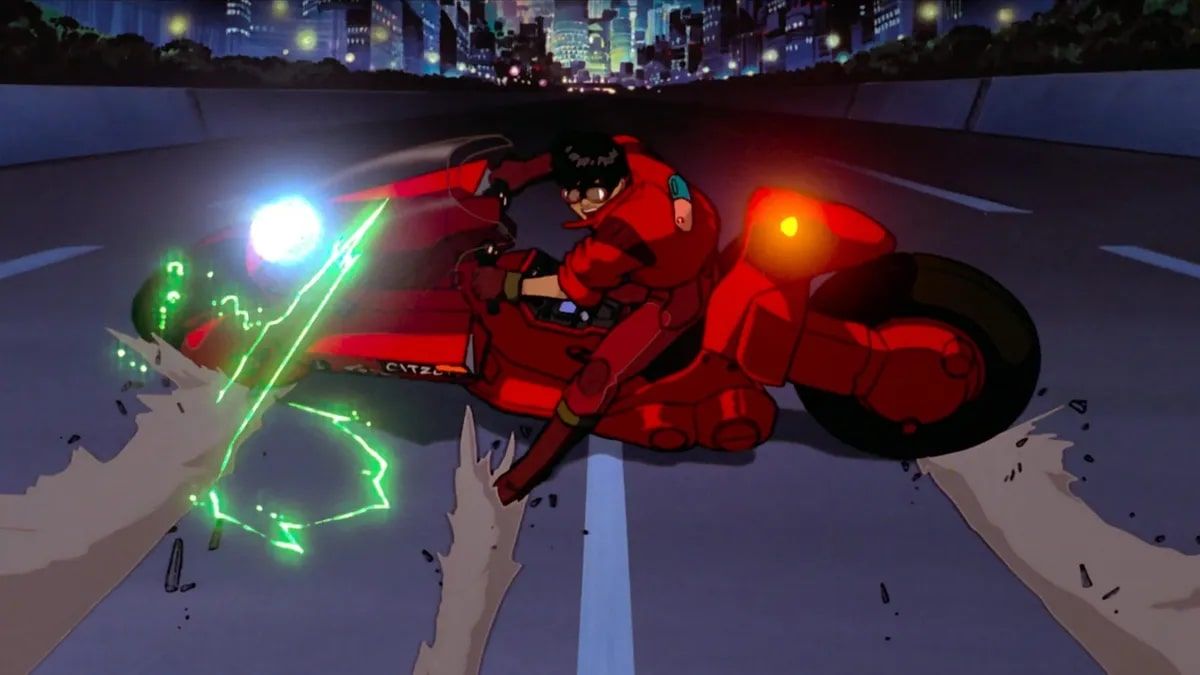
\includegraphics[scale=0.2]{../figures/akira.jpg}
    \caption{Escena de la película \textit{Akira} mostrando a Kaneda montando su motocicleta en la autopista de \textit{Neo-Tokio}.}
    \label{fig:akira-bike}
\end{figure}

El vector promedio $\vec{m}_1$ de la \cref{fig:akira-bike}, su matriz de covarianza $\Sigma_1$, y su matriz de correlación $R_1$ son
\begin{align*}
    \vec{m}_1 & =
    \begin{bmatrix}
        0.2733 \\
        0.2133 \\
        0.2612 \\
    \end{bmatrix}, &
    \Sigma_1 & =
    \begin{bmatrix}
        0.0295 & 0.0173 & 0.0135 \\
        0.0173 & 0.0331 & 0.0306 \\
        0.0135 & 0.0306 & 0.0360 
    \end{bmatrix}, &
    R_1 & = 
    \begin{bmatrix}
        1.0    & 0.5548 & 0.4164 \\
        0.5548 & 1.0    & 0.8869 \\
        0.4164 & 0.8869 & 1.0
    \end{bmatrix}.
\end{align*}

Los eigenvalores de $\Sigma_1$ son $\lambda_1 = 0.0033$, $\lambda_2 = 0.0197$, $\lambda_3 = 0.0756$, y sus respectivos eigenvectores son,
\begin{align*}
    \vec{u_1} & =
    \begin{bmatrix}
        0.1694 \\
        -0.7530 \\
        0.6357
    \end{bmatrix}, &
    \vec{u_2} & = 
    \begin{bmatrix}
        0.8875 \\
        -0.1638 \\
        -0.4306
    \end{bmatrix}, &
    \vec{u_3} & =
    \begin{bmatrix}
        0.4284 \\
        0.6372 \\
        0.6406
    \end{bmatrix}.
\end{align*}

% angulos para imagenes [-0.3, 0.3, 0.65]
La nube de pixeles de la \cref{fig:akira-bike} se muestra en la \cref{fig:nube-pixeles-akira} con 3 angulos de vista distintos para poder observar mejor la nube y su vector promedio. También se incluyen los eigenvectores de la imagen a partir del vector promedio.
\begin{figure}[ht!]
    \centering
    \begin{subfigure}[c]{0.3\textwidth}
        \centering
        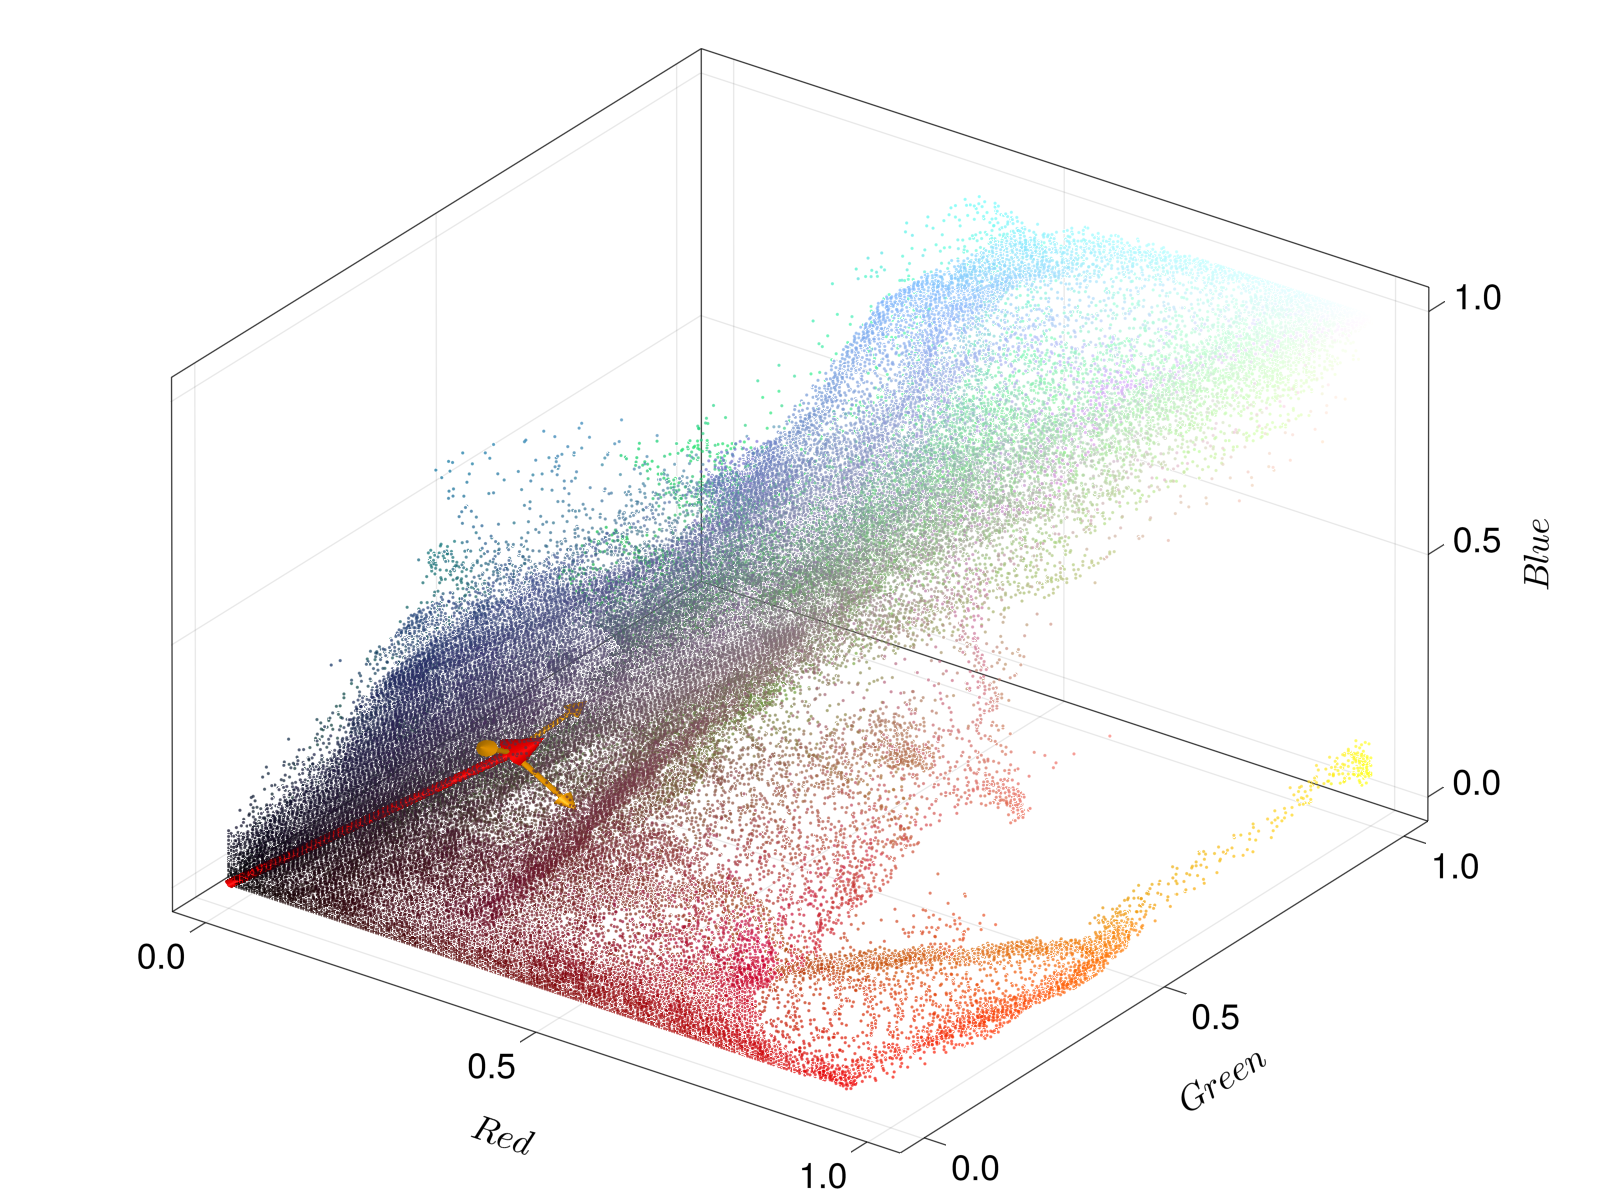
\includegraphics[scale=0.09]{../figures/pixel_cloud_akira_1}
    \end{subfigure}
    \begin{subfigure}[c]{0.3\textwidth}
        \centering
        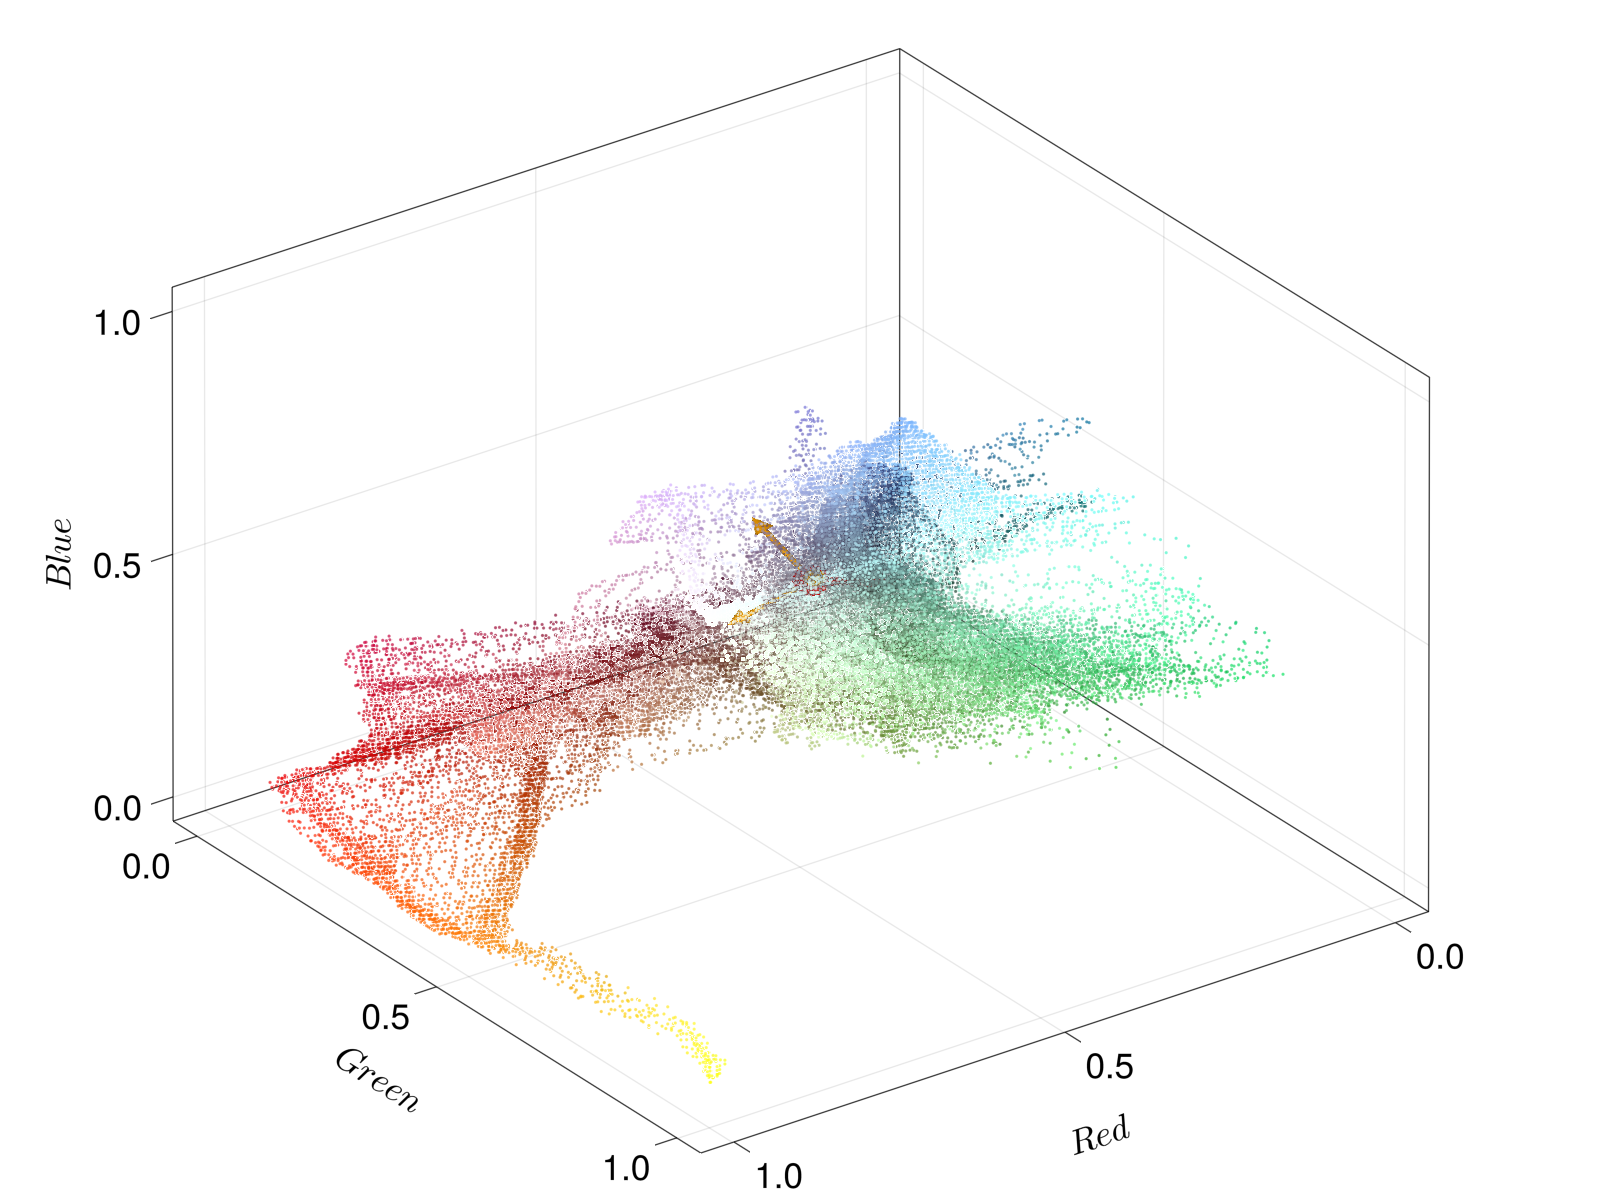
\includegraphics[scale=0.09]{../figures/pixel_cloud_akira_2}
    \end{subfigure}
    \begin{subfigure}[c]{0.3\textwidth}
        \centering
        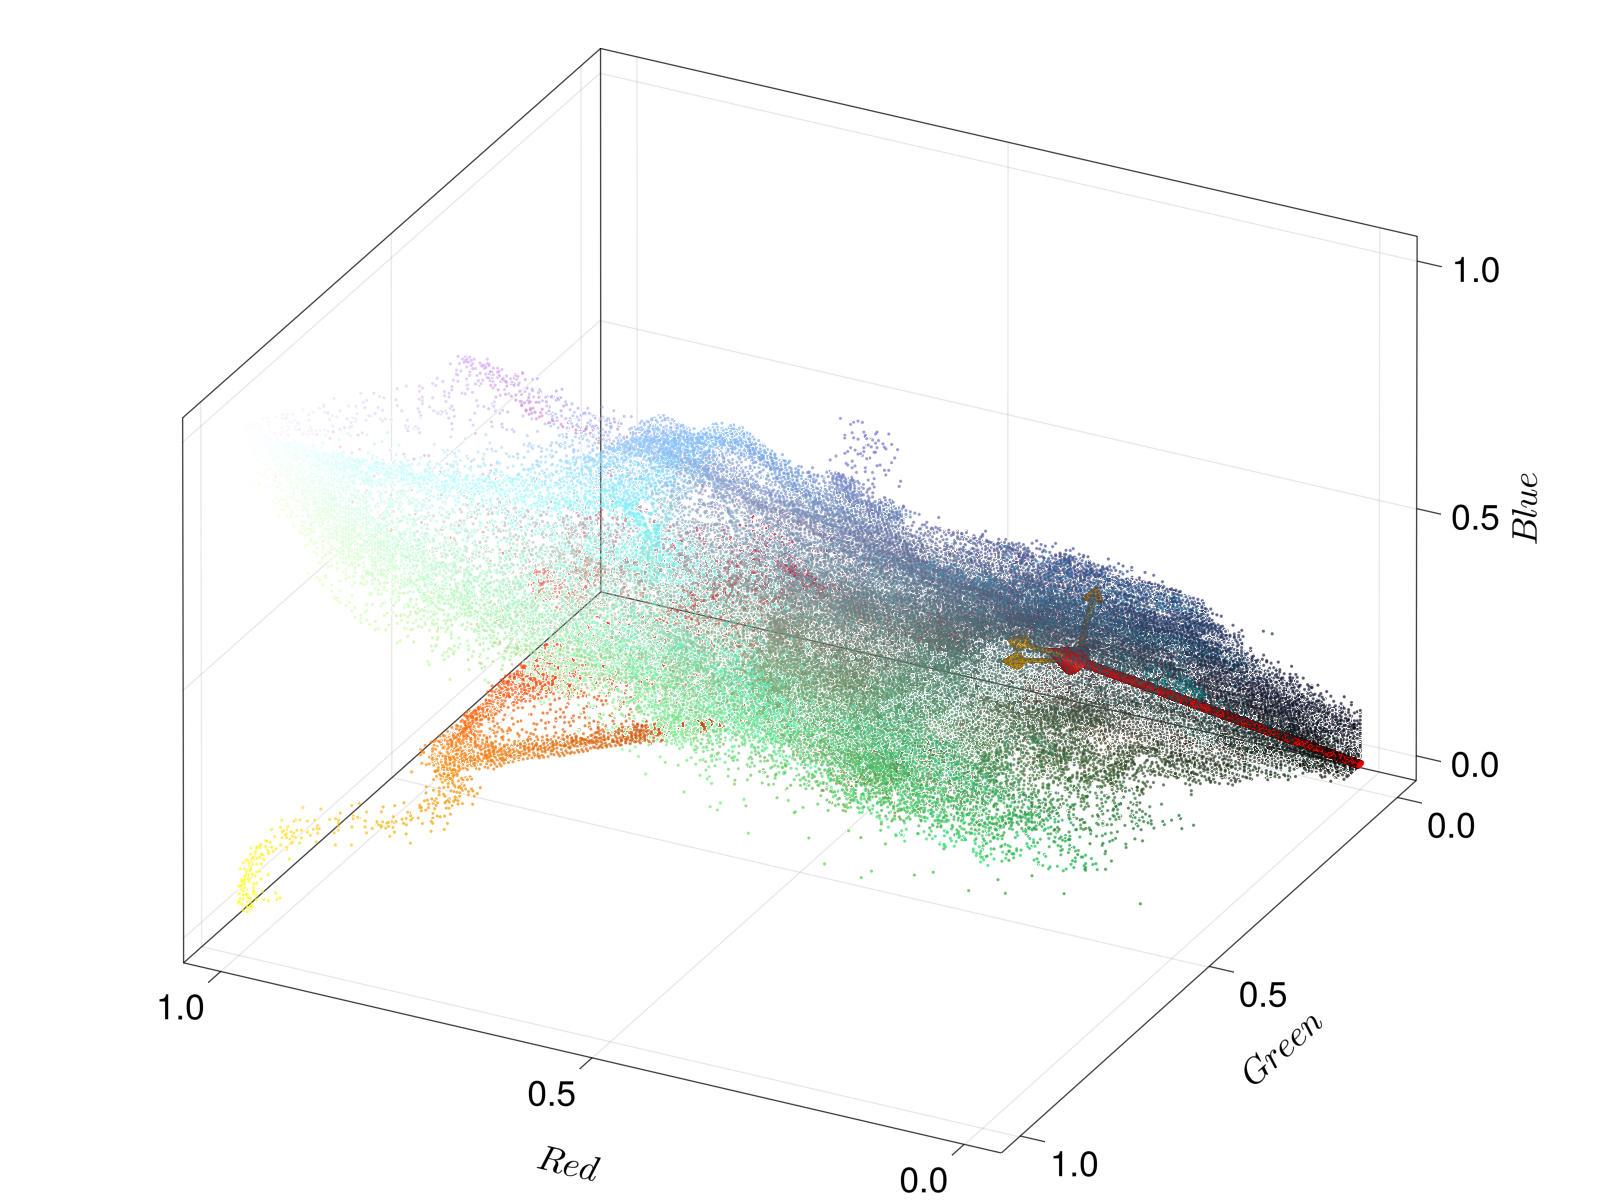
\includegraphics[scale=0.09]{../figures/pixel_cloud_akira_3}
    \end{subfigure}
    \caption{Nubes de pixeles para la de la \cref{fig:akira-bike}, donde se muestran con una rotación respecto al eje-$Blue$ de la vista de $-0.3\pi$, $0.3\pi$, y $0.65\pi$, respectivamente.}
    \label{fig:nube-pixeles-akira}
\end{figure}

Para realizar estas gráficas de manera más eficiente se obtuvo el conjunto de puntos RGB únicos de la imágen ya que si alguno de ellos se repetía sería sobrepuesto donde ya hay un pixel ubicado. Esto se hizo únicamente con propósitos visuales y no para computar $\vec{m}$, ni la matriz de covarianza ni la de correlación.

Además de las nubes de pixeles se decidó graficar un espacio de probabilidad de puntos discretos $(r,g,b)$ donde las tres coordenadas pueden tomar valores dentro del rango $[0,1]$.
\begin{figure}[ht!]
    \centering
    \begin{subfigure}[c]{0.3\textwidth}
        \centering
        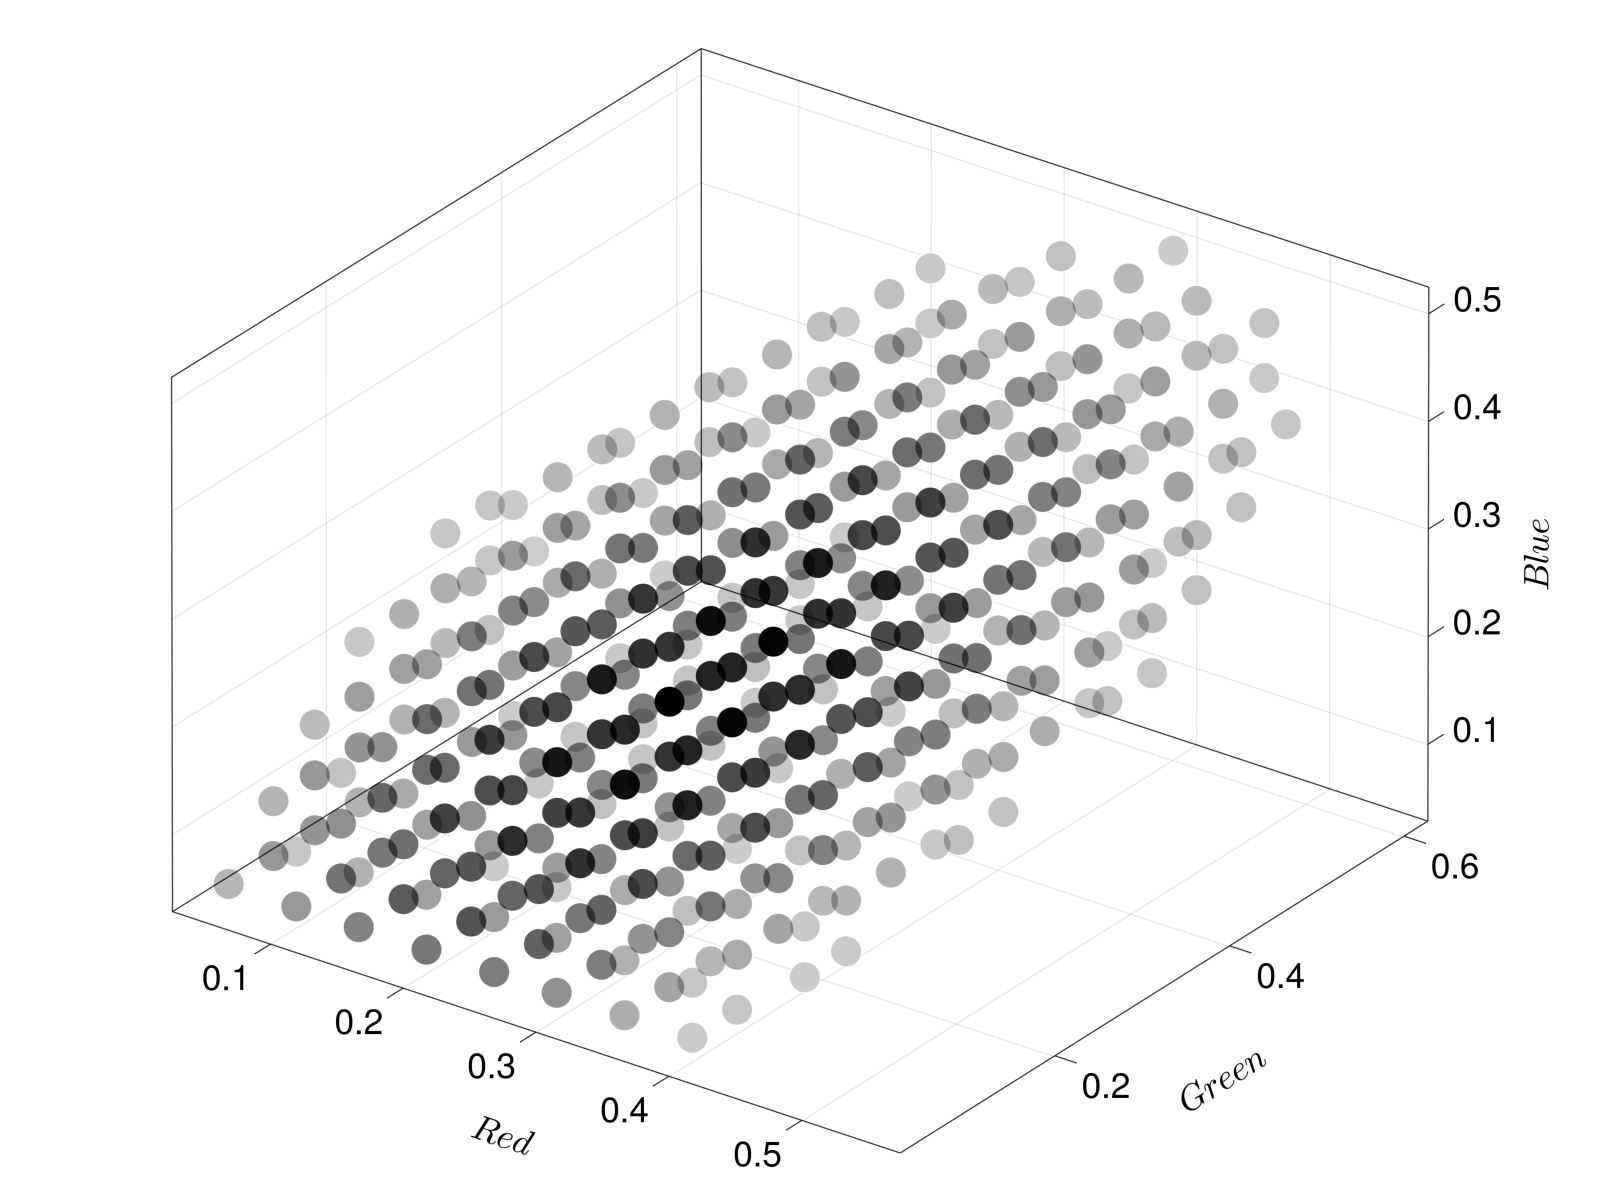
\includegraphics[scale=0.09]{../figures/gaussian_cloud_akira_1}
    \end{subfigure}
    \begin{subfigure}[c]{0.3\textwidth}
        \centering
        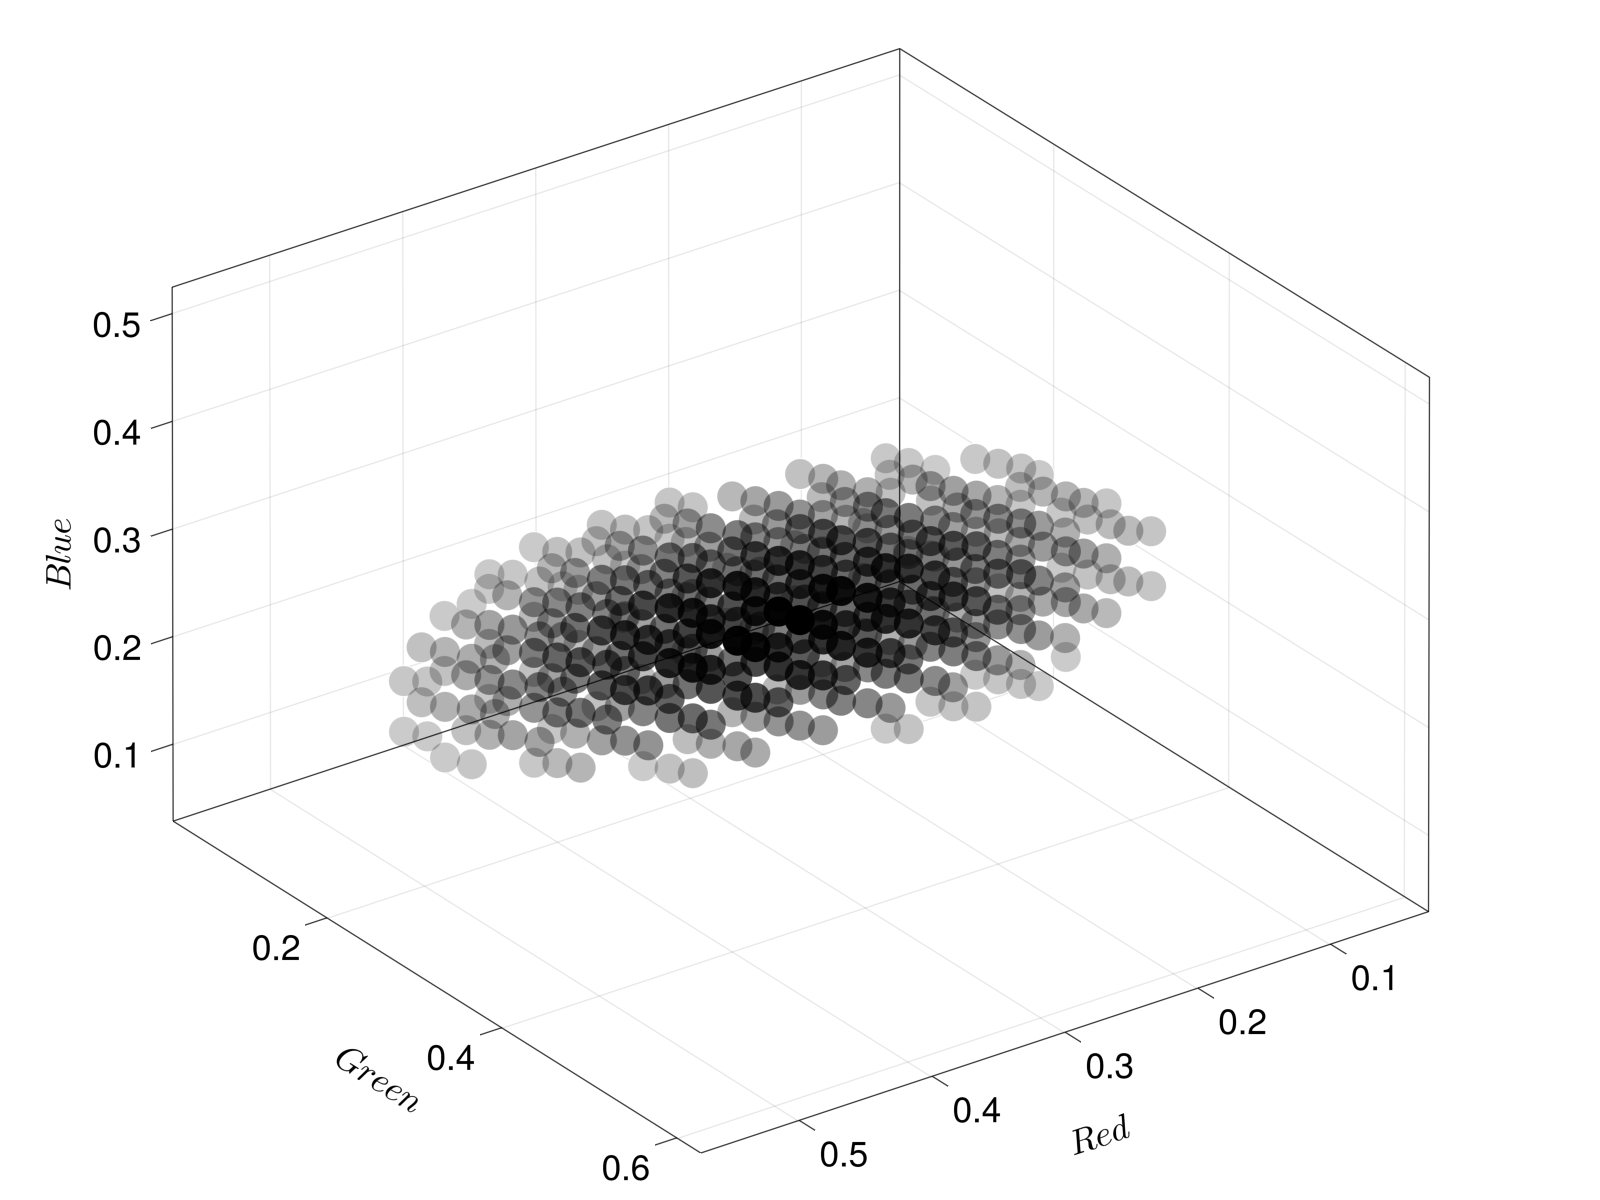
\includegraphics[scale=0.09]{../figures/gaussian_cloud_akira_2}
    \end{subfigure}
    \begin{subfigure}[c]{0.3\textwidth}
        \centering
        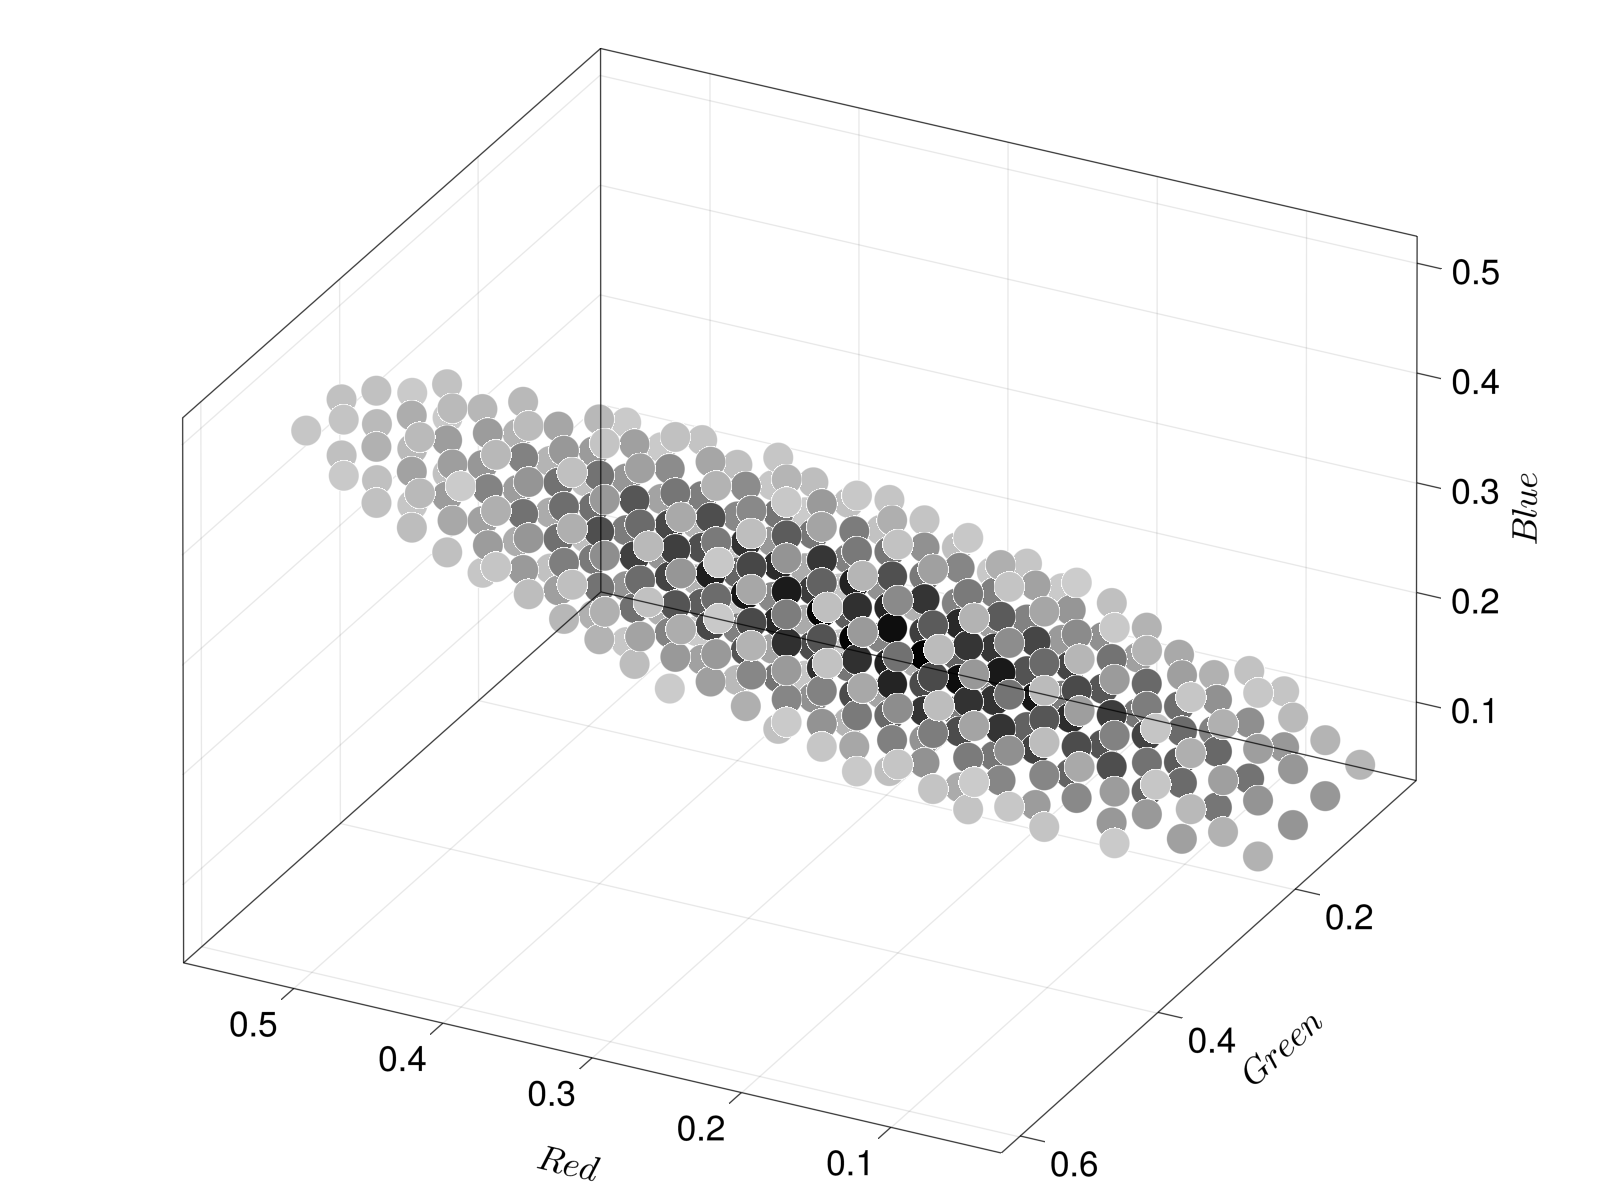
\includegraphics[scale=0.09]{../figures/gaussian_cloud_akira_3}
    \end{subfigure}
    \caption{Nubes de probabilidad para la \cref{fig:akira-bike}, donde se muestran con una rotación respecto al eje-$Blue$ de la vista de $-0.3\pi$, $0.3\pi$, y $0.65\pi$, respectivamente.}
    \label{fig:nube-gaussiana-akira}
\end{figure}
La ecuación que se usó para las nubes gaussianas de probabilidad es
\begin{equation}
    \mathcal{N}(\vec{x}|\vec{\mu}, \Sigma) = \frac{1}{(2 \pi)^{D/2} |\Sigma|^{1/2}} \exp\left\{-\frac{1}{2} (\vec{x} - \vec{\mu})^{t} \Sigma^{-1} (\vec{x} - \vec{\mu}) \right\}\ ,
\end{equation}
donde $D$ es la dimensión de los vectores $\vec{x}$ y $\vec{\mu}$, y la matriz $\Sigma$ tiene dimensión $D \times D$.

La segunda imagen que se utilizó es una pintura hecha por el artista \href{https://twitter.com/DaBroque}{Kate da Broque}\footnote{https://linktr.ee/katedabroque}. Esta imagen se muestra en la \cref{fig:kate-da-broque}, tiene aproximadamente $1.2E7$ pixeles y las dimensiones de la imagen son $(4096, 2958)$.
\begin{figure}[ht!]
    \centering
    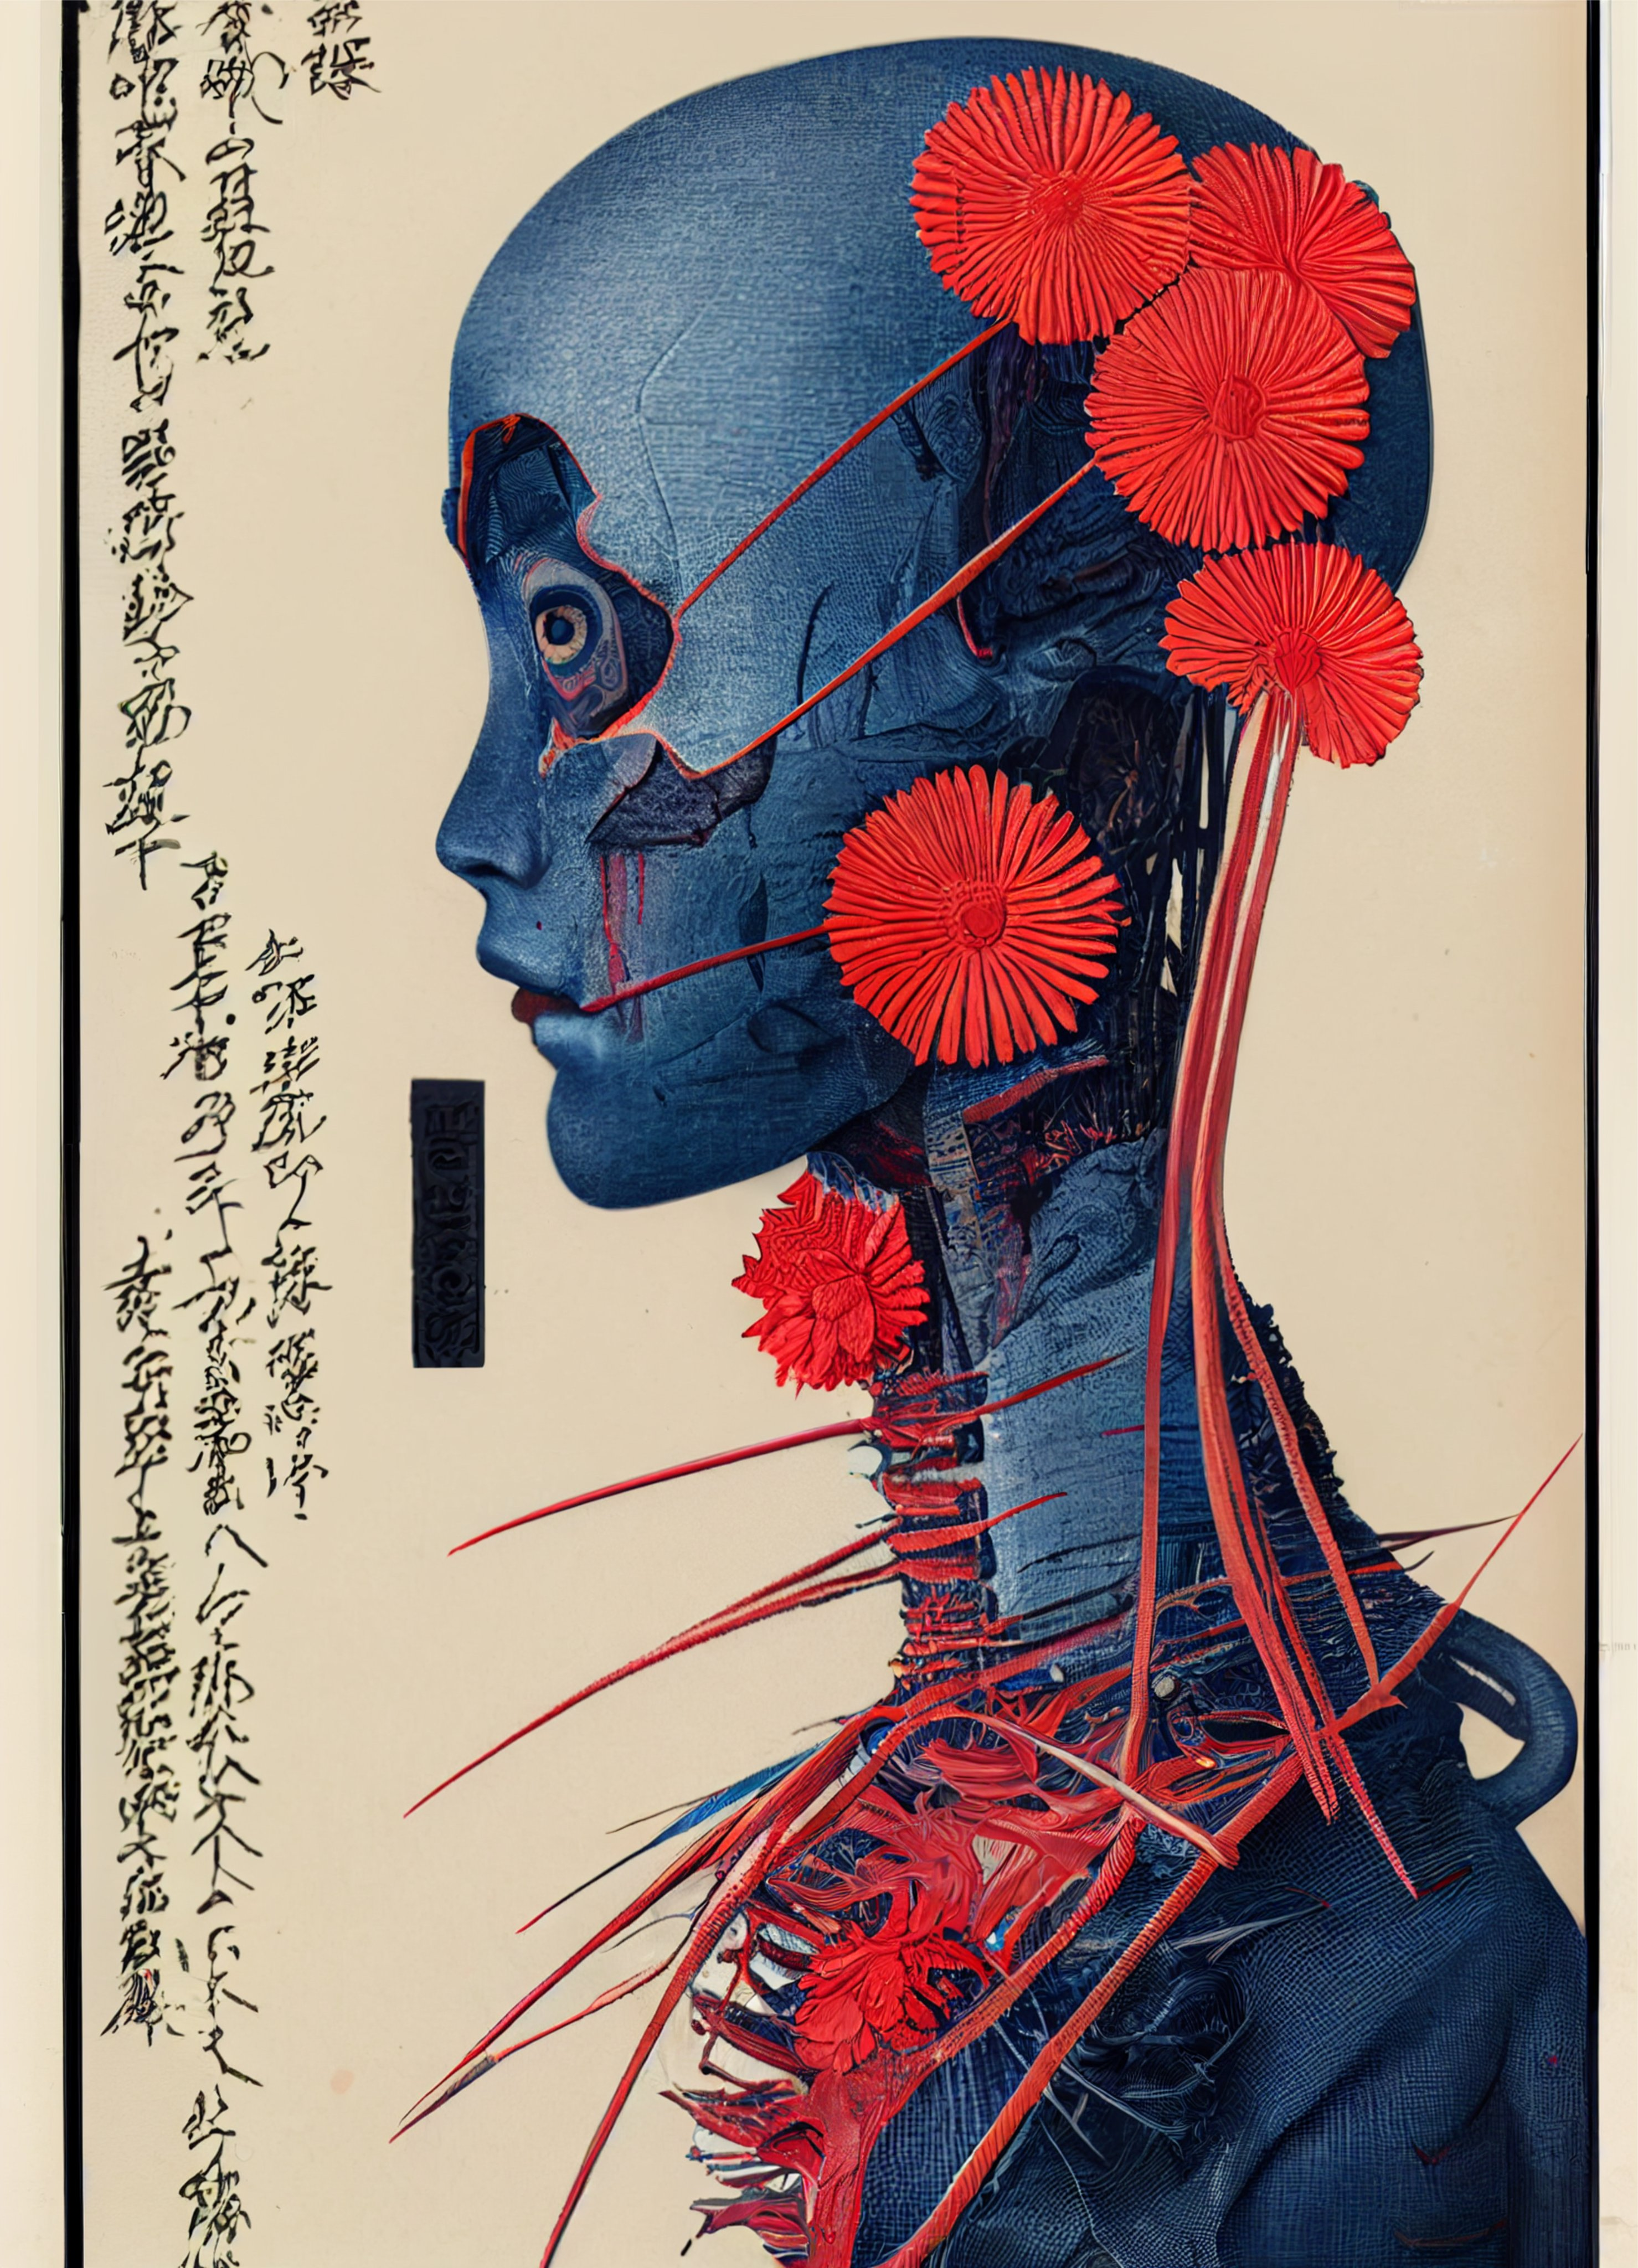
\includegraphics[scale=0.05]{../figures/kate-da-broque}
    \caption{Obra por el artista Kate da Broque titulada \textit{japanoid android}.}
    \label{fig:kate-da-broque}
\end{figure}

El vector promedio $\vec{m}_2$, la matriz de covarianza $\Sigma_2$ y la matriz de correlación $R_2$ de la \cref{fig:kate-da-broque} son,
\begin{align*}
    \vec{m}_2 & =
    \begin{bmatrix}
        0.6010 \\
        0.5114 \\
        0.4940
    \end{bmatrix}, &
    \Sigma_2 & =
    \begin{bmatrix}
        0.1199 & 0.0882 & 0.0606 \\
        0.0882 & 0.1030 & 0.0784 \\
        0.0606 & 0.0784 & 0.0627
    \end{bmatrix}, &
    R_2 & = 
    \begin{bmatrix}
        1.0    & 0.7943 & 0.6992 \\
        0.7943 & 1.0    & 0.9760 \\
        0.6992 & 0.9760 & 1.0
    \end{bmatrix}.
\end{align*}

Los eigenvalores de $\Sigma_2$ son $\lambda_1 = 0.0010$, $\lambda_2 = 0.0334$, $\lambda_3 = 0.2511$, y sus respectivos eigenvectores son
\begin{align*}
    \vec{v_1} & =
    \begin{bmatrix}
        0.1259 \\
        -0.6713 \\
        0.7304
    \end{bmatrix}, &
    \vec{v_2} & = 
    \begin{bmatrix}
        0.7645 \\
        -0.4034 \\
        -0.5026
    \end{bmatrix}, &
    \vec{v_3} & =
    \begin{bmatrix}
        0.6321 \\
        0.6217 \\
        0.4624
    \end{bmatrix}.
\end{align*}

La nube de pixeles, con su vector promedio y eigenvectores, de la \cref{fig:kate-da-broque} se muestran en la \cref{fig:nube-pixeles-kate}.
\begin{figure}[ht!]
    \centering
    \begin{subfigure}[c]{0.3\textwidth}
        \centering
        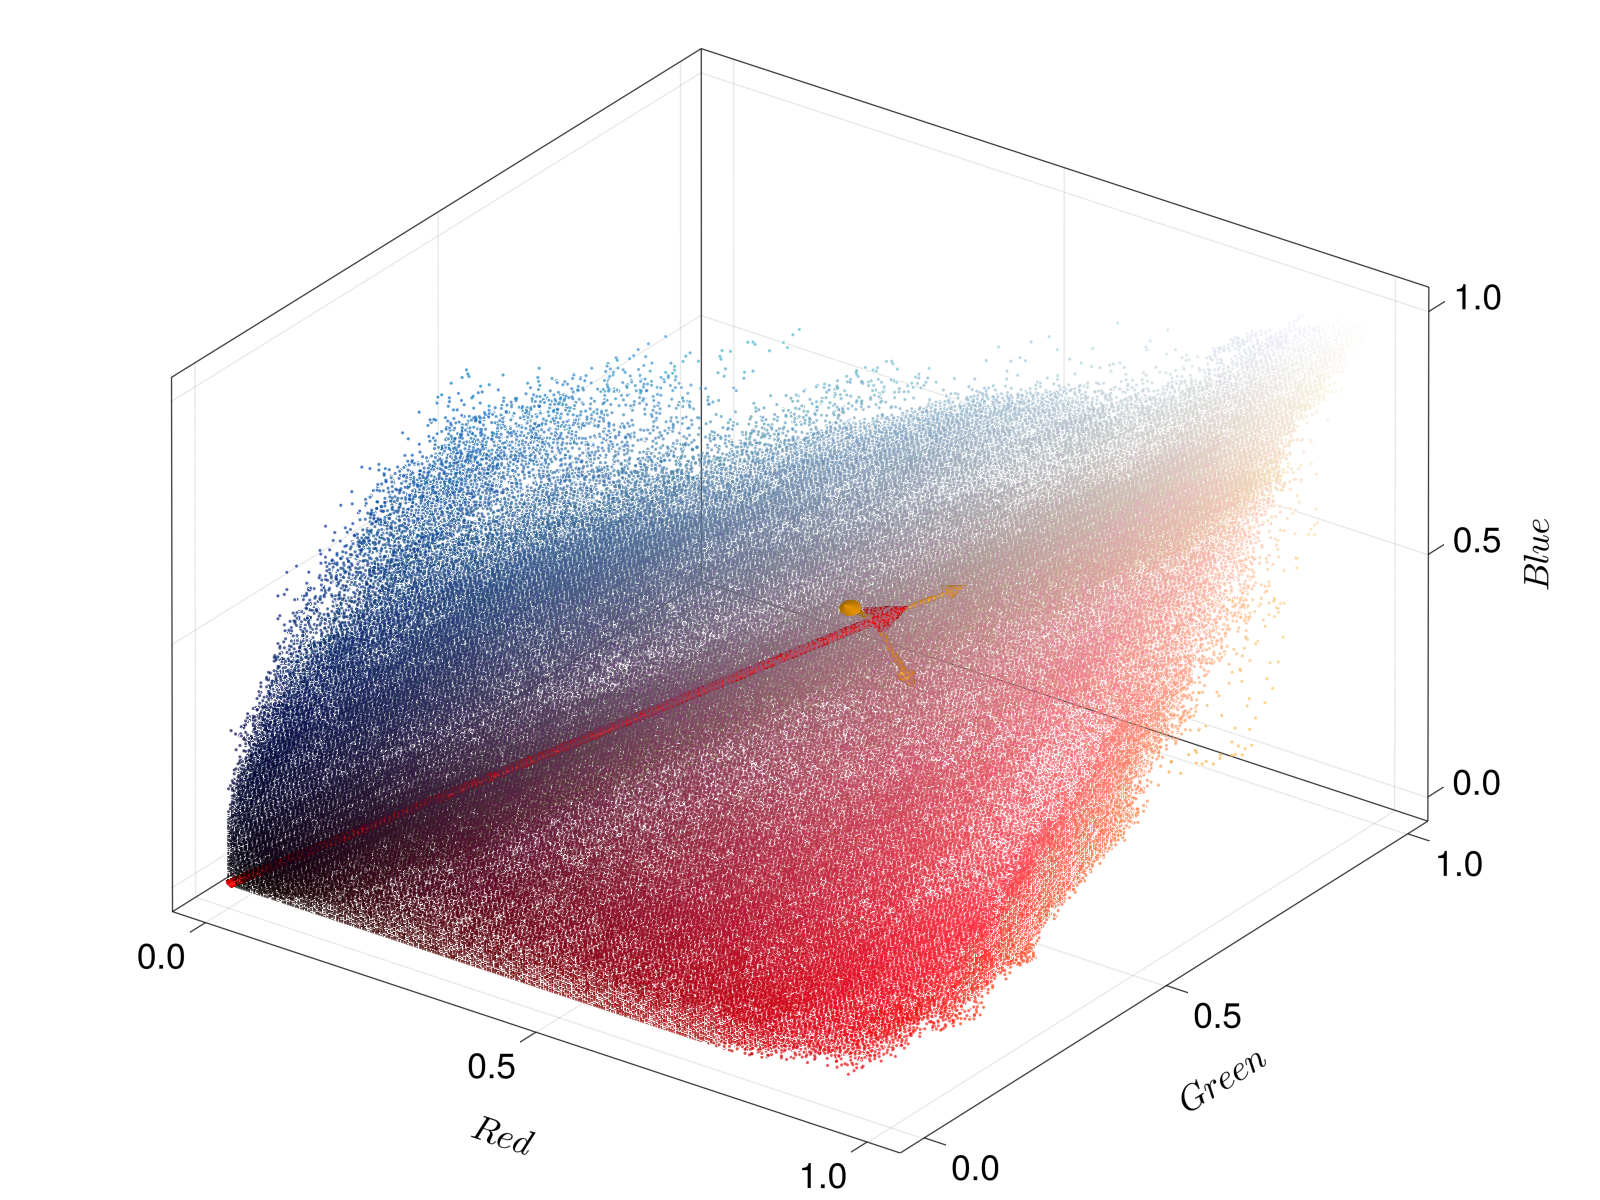
\includegraphics[scale=0.09]{../figures/pixel_cloud_kate_1}
    \end{subfigure}
    \begin{subfigure}[c]{0.3\textwidth}
        \centering
        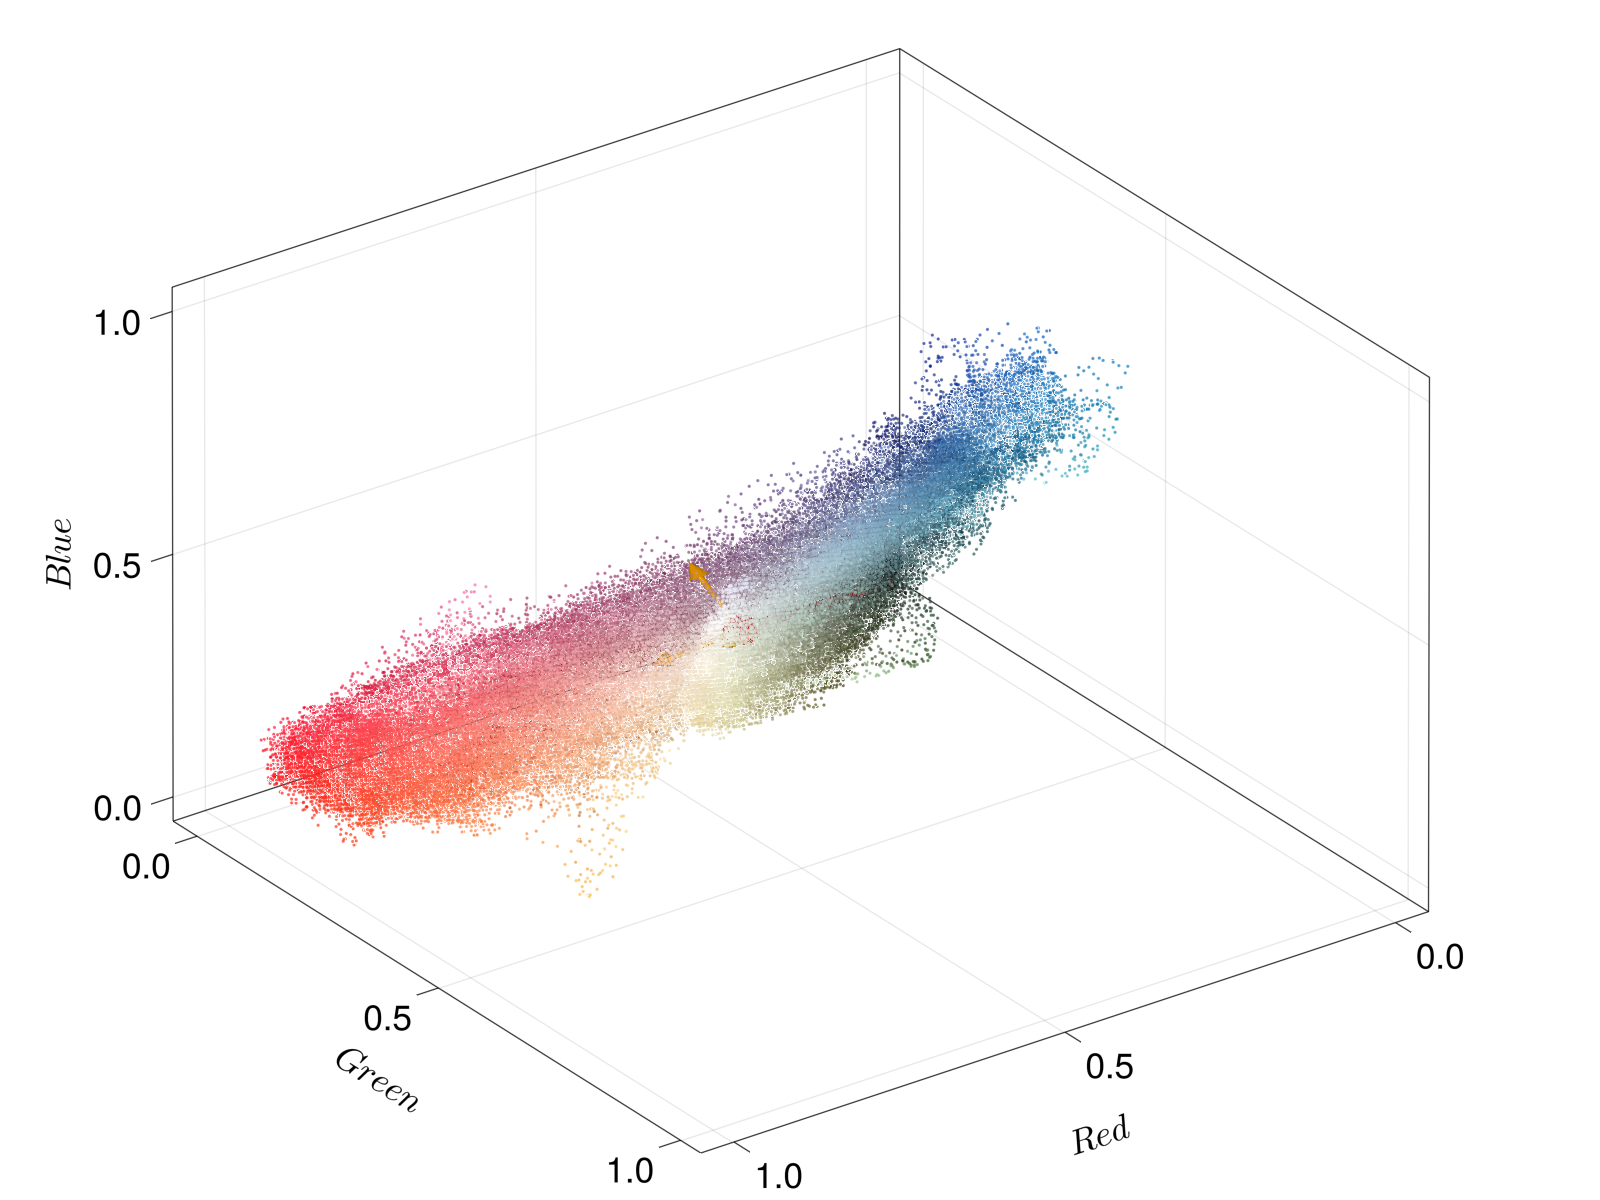
\includegraphics[scale=0.09]{../figures/pixel_cloud_kate_2}
    \end{subfigure}
    \begin{subfigure}[c]{0.3\textwidth}
        \centering
        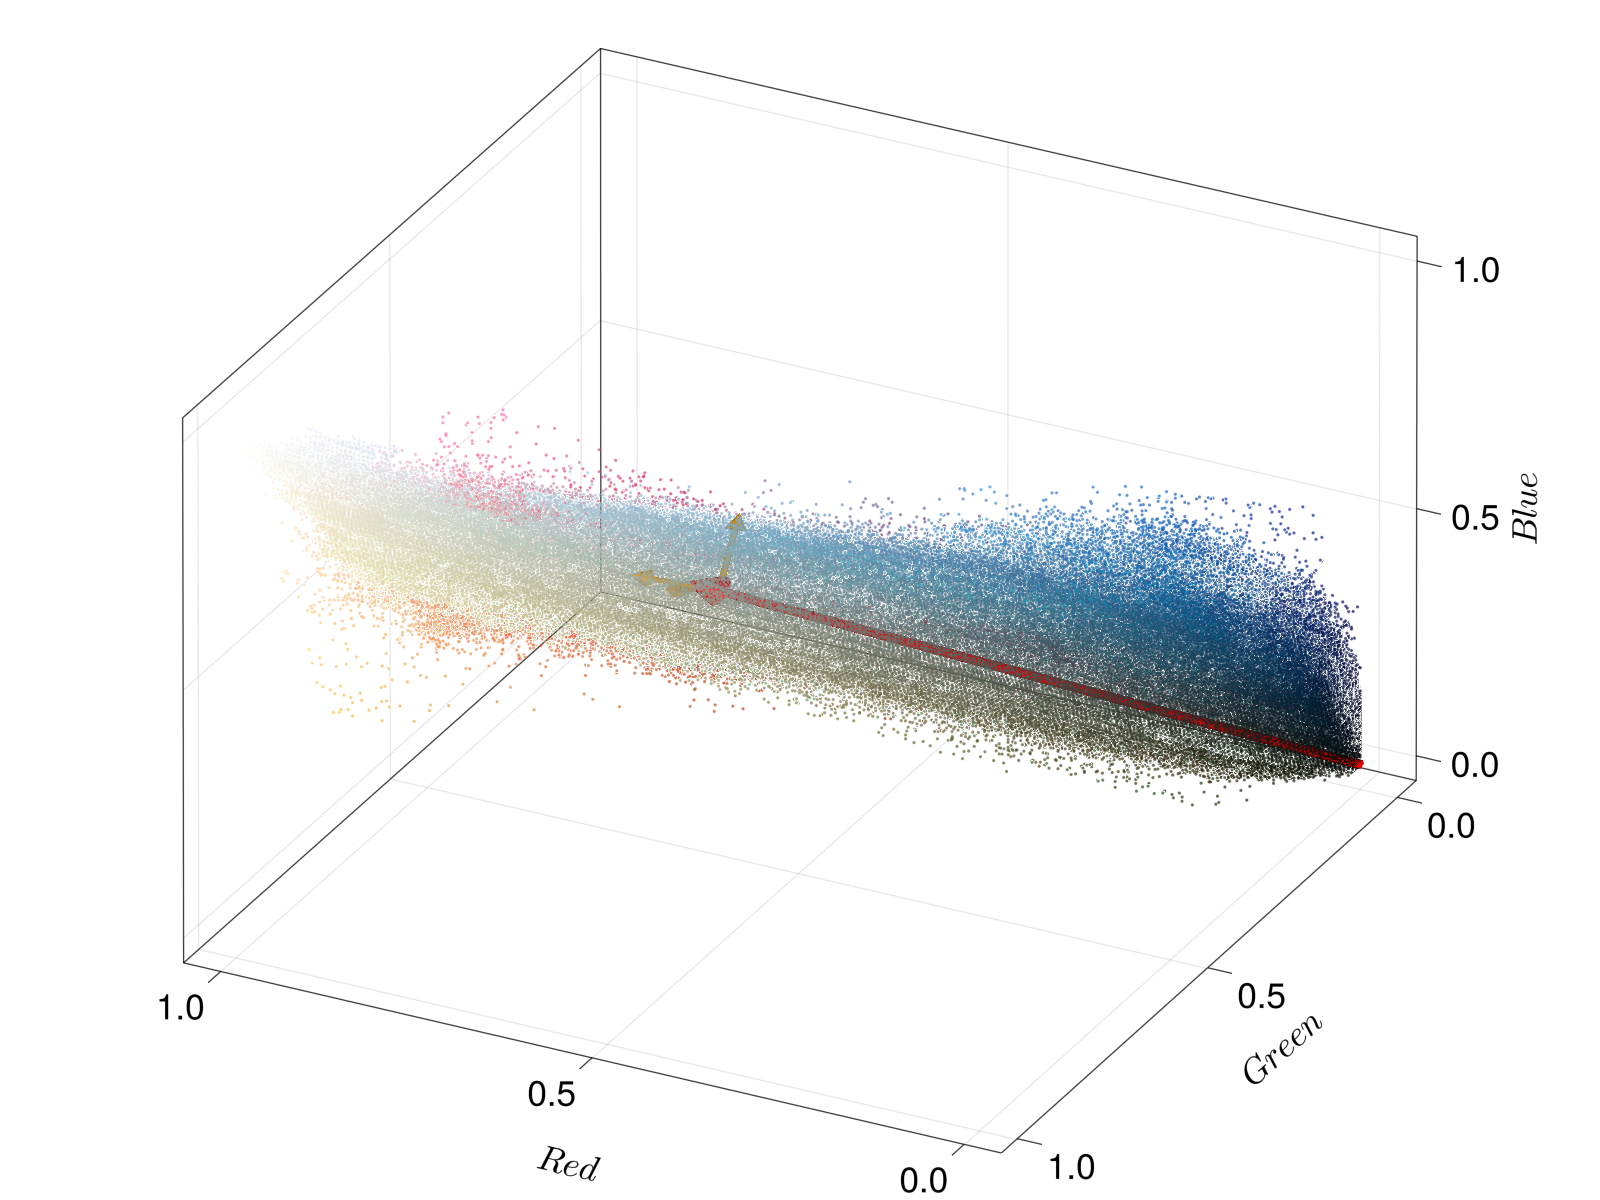
\includegraphics[scale=0.09]{../figures/pixel_cloud_kate_3}
    \end{subfigure}
    \caption{Nubes de pixeles para la \cref{fig:kate-da-broque} con angulos de rotación para las vistas respecto al eje-$Blue$ de $-0.3\pi$, $0.3\pi$ y $0.65\pi$, respectivamente.}
    \label{fig:nube-pixeles-kate}
\end{figure}

Las nubes de probabilidad para la \cref{fig:kate-da-broque} se muestran en la \cref{fig:nube-gaussiana-kate}. Para este caso, la nube de probabilidad se encuentra concentrada y achatada en la dirección del vector promedio $\vec{m}_2$ lo cual tiene sentido si se observa la distribucion de la nube de pixeles.
\begin{figure}[ht!]
    \centering
    \begin{subfigure}[c]{0.3\textwidth}
        \centering
        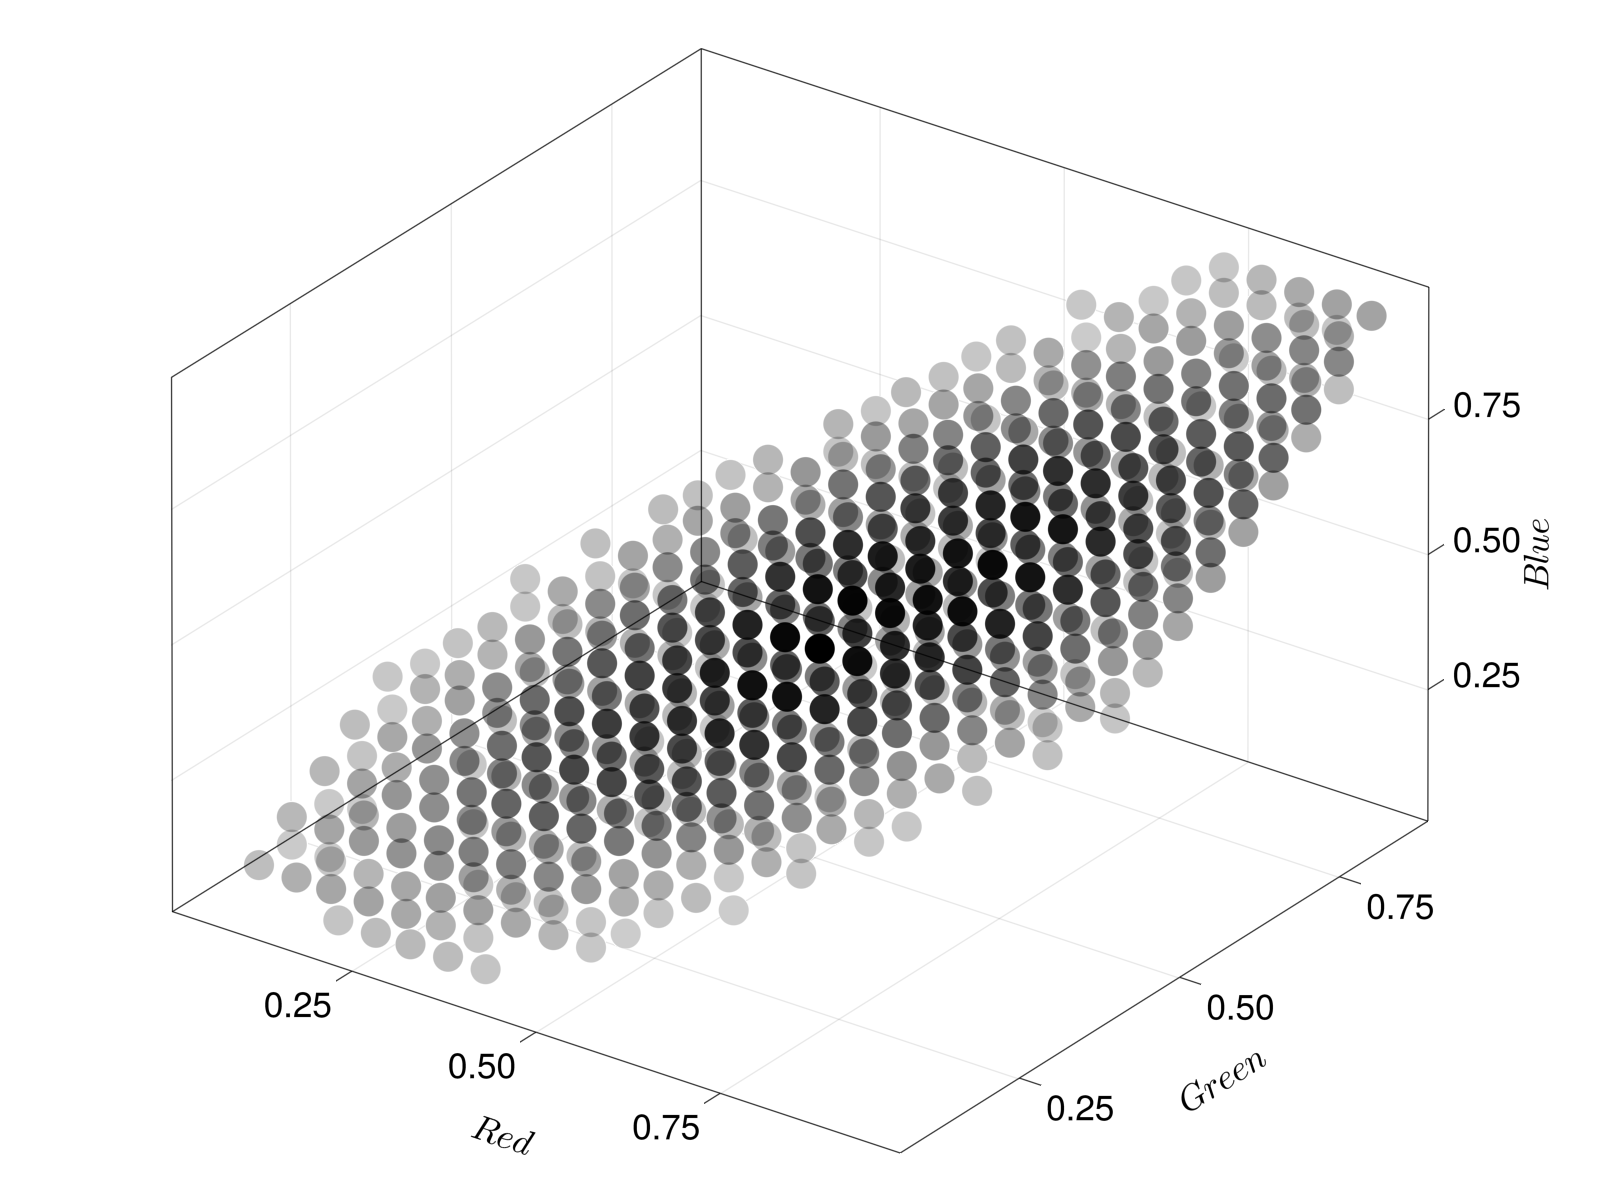
\includegraphics[scale=0.09]{../figures/gaussian_cloud_kate_1}
    \end{subfigure}
    \begin{subfigure}[c]{0.3\textwidth}
        \centering
        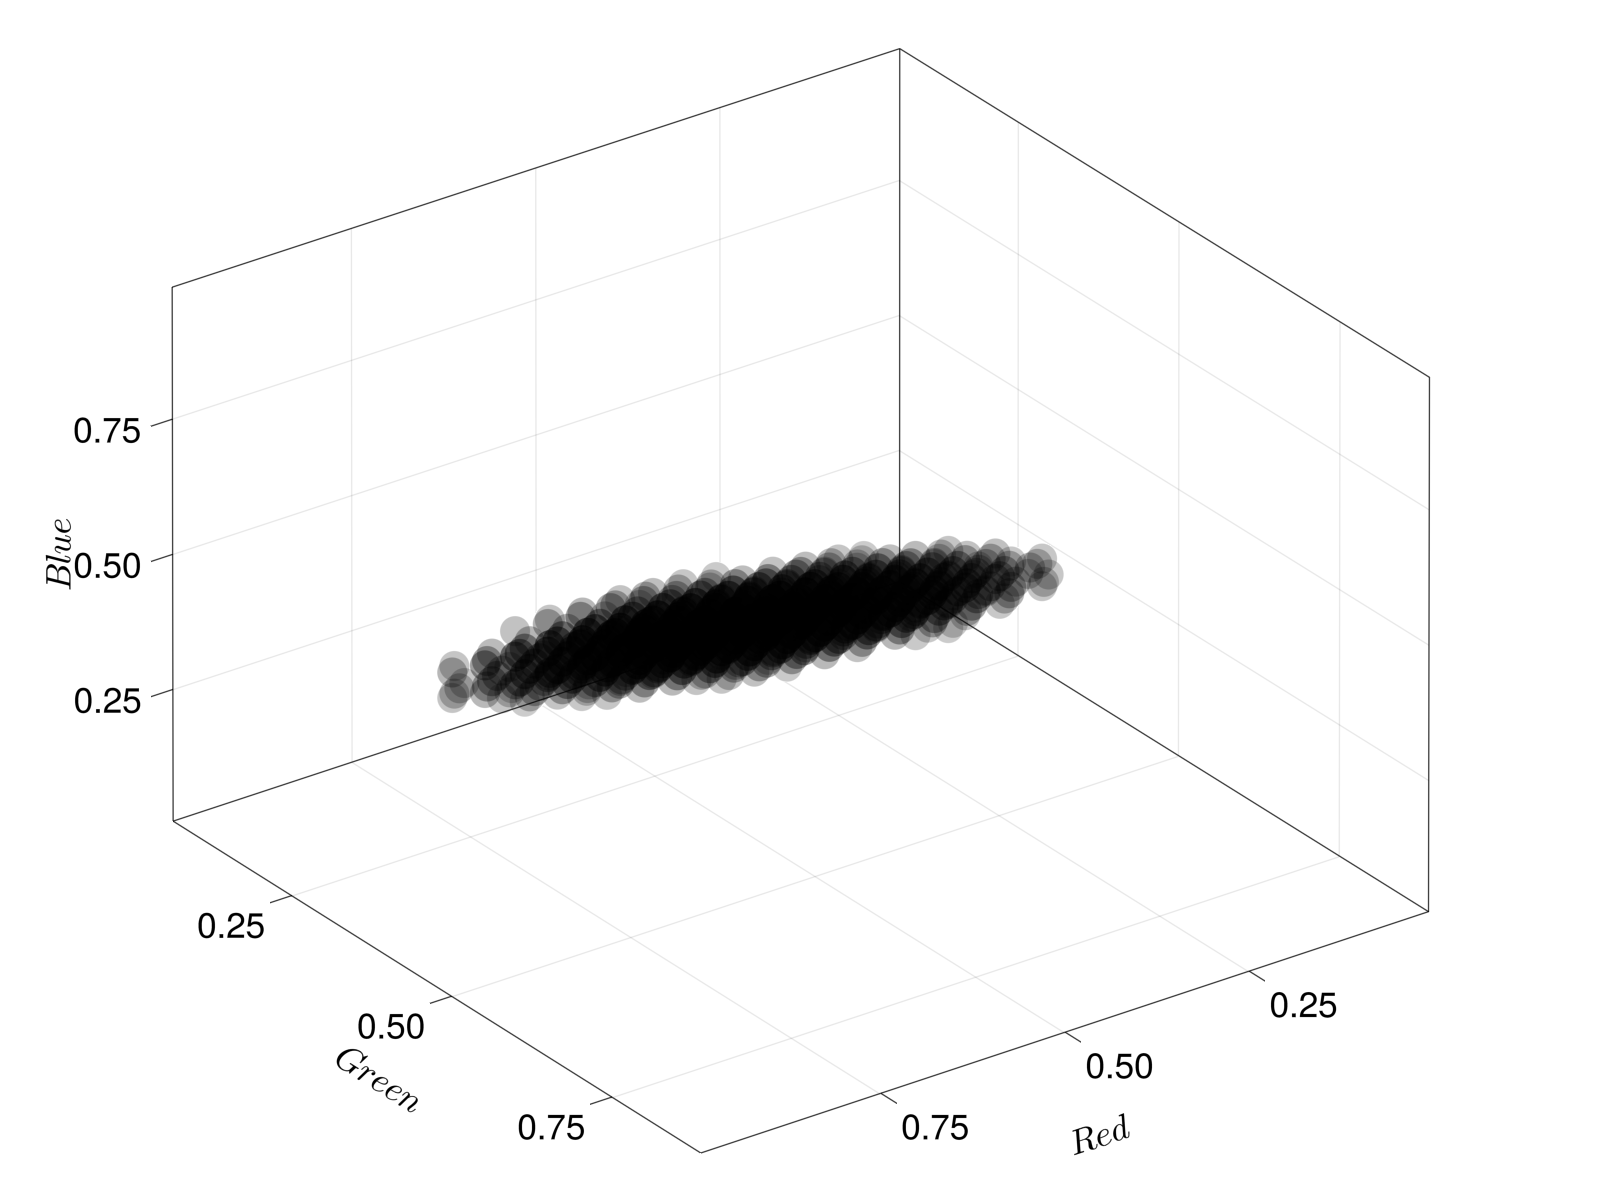
\includegraphics[scale=0.09]{../figures/gaussian_cloud_kate_2}
    \end{subfigure}
    \begin{subfigure}[c]{0.3\textwidth}
        \centering
        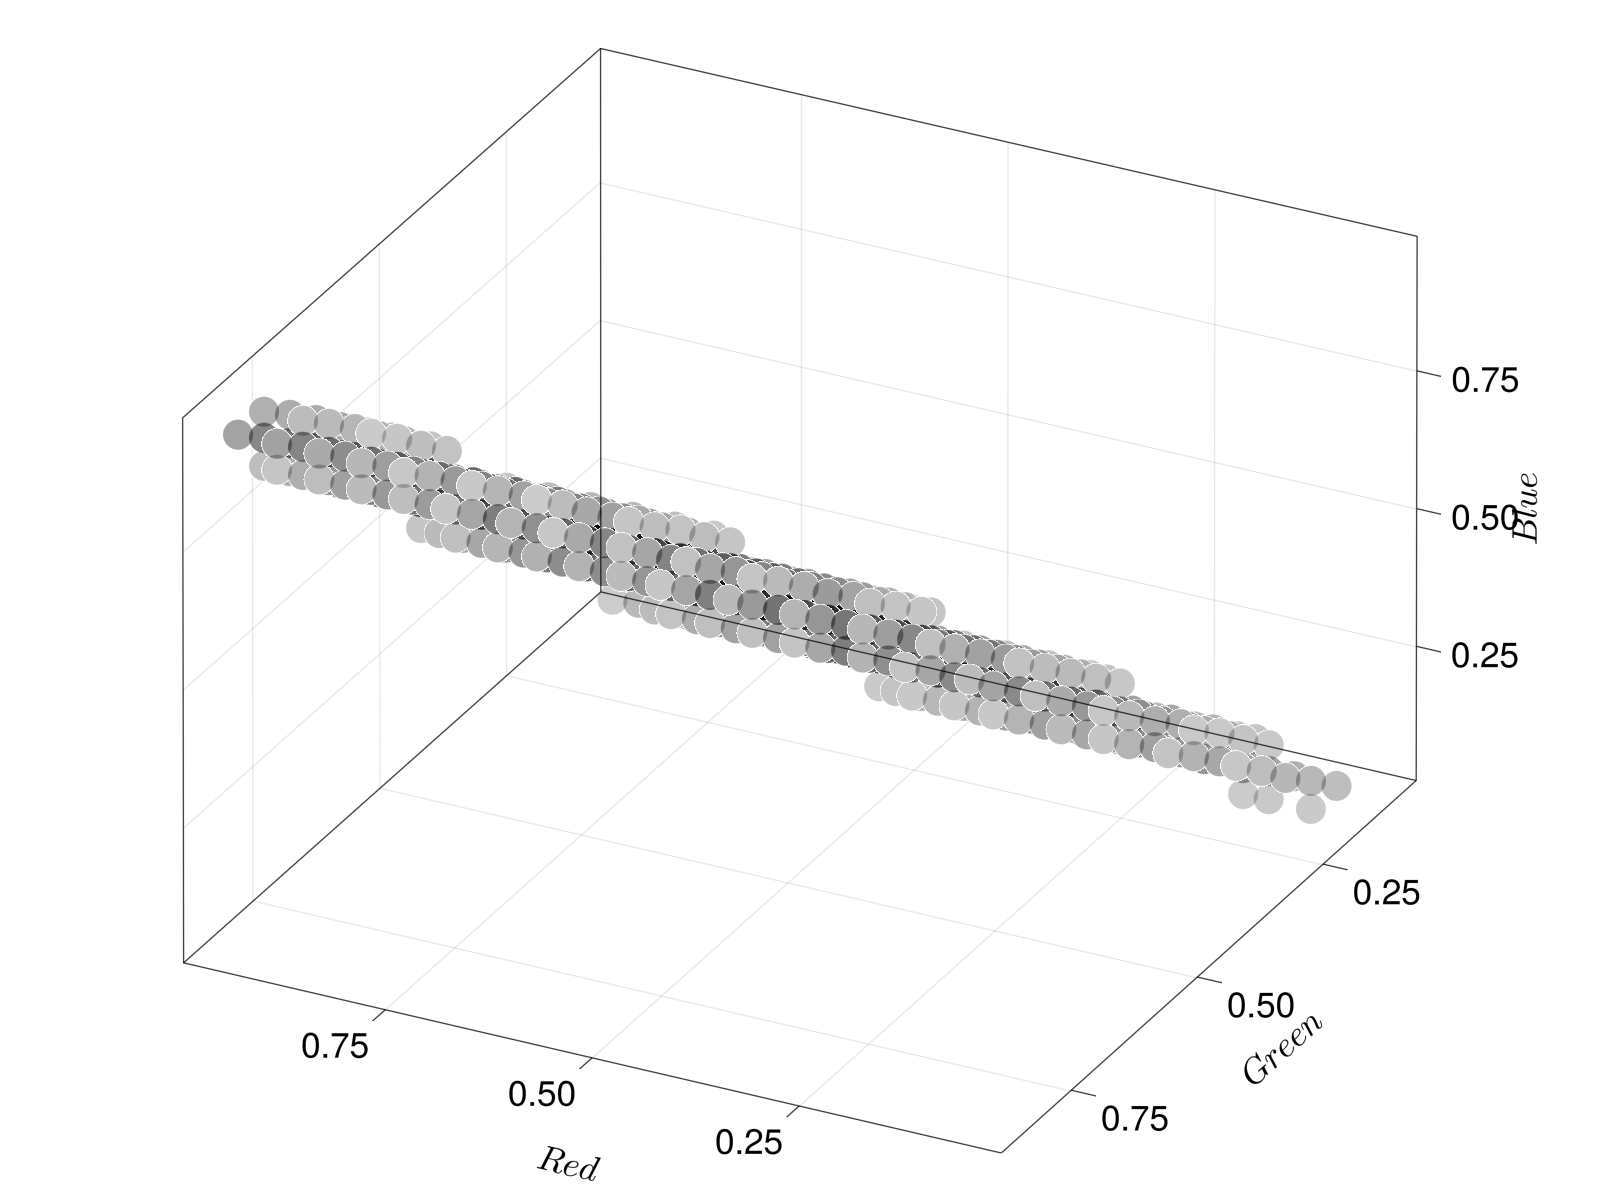
\includegraphics[scale=0.09]{../figures/gaussian_cloud_kate_3}
    \end{subfigure}
    \caption{Nubes de probabilidad para la \cref{fig:kate-da-broque}, donde se muestran con una rotación respecto al eje-$Blue$ de la vista de $-0.3\pi$, $0.3\pi$, y $0.65\pi$, respectivamente.}
    \label{fig:nube-gaussiana-kate}
\end{figure}

Tanto las nubes de probabilidad en la \cref{fig:nube-gaussiana-akira} y la \cref{fig:nube-gaussiana-kate} son muy parecidas, mientras que una está mas achatada que la otra ¿Qué pasaría si forzaramos de alguna manera a la nube de probabilidad en otra dirección? Para responder a esta pregunta basta con elegir una imagen que muchos de sus pixeles se inclinen a un color en particular. Se eligió una toma en específico de la película \textit{Evangelion: 3.0+1.0 Thrice Upon a Time} \cite{hideaki2022eva} donde el color rojo predomina en toda la escena.
\begin{figure}[ht!]
    \centering
    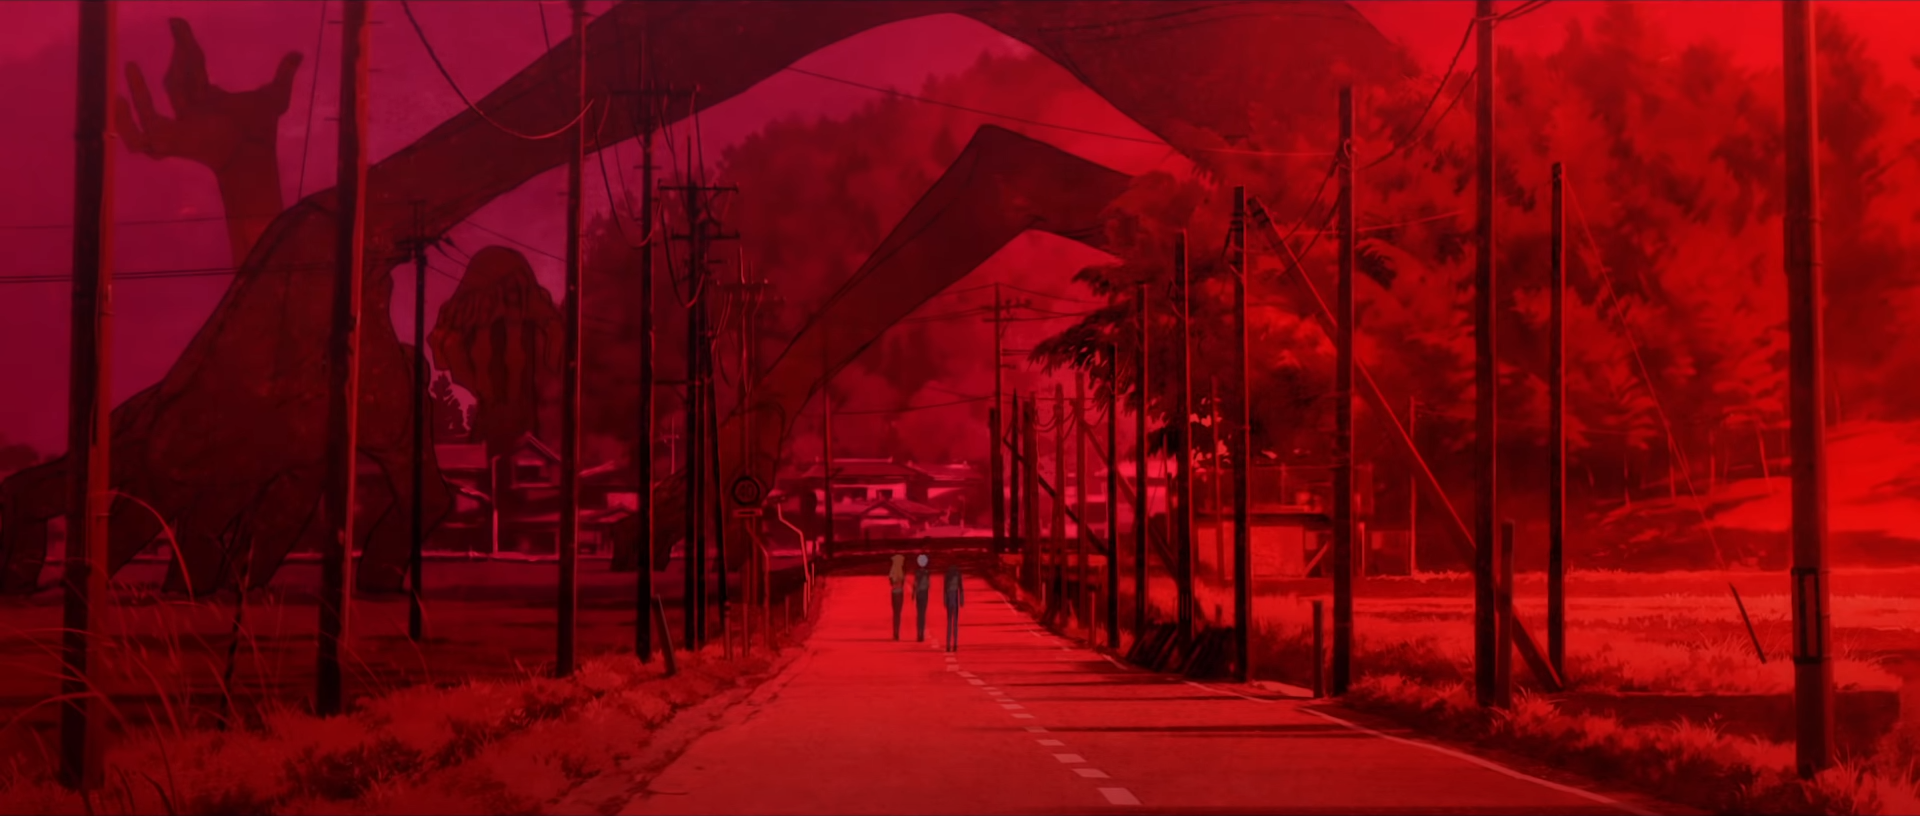
\includegraphics[scale=0.2]{../figures/evangelion}
    \caption{Imagen donde predomina el color al rojo.}
    \label{fig:evangelion}
\end{figure}

La imagen mostrada en la \cref{fig:evangelion} tiene aproximadamente $1.5E6$ pixeles, y sus dimensiones son $(816, 1920)$. El vector promedio $\vec{m}_3$, la matriz de covarianza $\Sigma_3$ y la matriz de correlación $R_3$ de la \cref{fig:evangelion} son
\begin{align*}
    \vec{m}_3 & =
    \begin{bmatrix}
        0.4561 \\
        0.0258 \\
        0.0539
    \end{bmatrix}, &
    \Sigma_3 & =
    \begin{bmatrix}
        0.0342 & 0.0031 & 0.0041 \\
        0.0031 & 0.0006 & 0.0008 \\
        0.0041 & 0.0008 & 0.0027
    \end{bmatrix}, &
    R_3 & = 
    \begin{bmatrix}
        1.0    & 0.6633 & 0.4354 \\
        0.6633 & 1.0    & 0.6567 \\
        0.4354 & 0.6567 & 1.0
    \end{bmatrix}.
\end{align*}

Los eigenvalores de $\Sigma_3$ son $\lambda_1 = 0.0002$, $\lambda_2 = 0.0022$, $\lambda_3 = 0.0351$, y sus respectivos eigenvectores son
\begin{align*}
    \vec{w_1} & =
    \begin{bmatrix}
        0.0603 \\
        -0.9672 \\
        0.2465
    \end{bmatrix}, &
    \vec{w_2} & = 
    \begin{bmatrix}
        -0.1494 \\
        0.2354 \\
        0.9603
    \end{bmatrix}, &
    \vec{w_3} & =
    \begin{bmatrix}
        0.9869 \\
        0.0947 \\
        0.1303
    \end{bmatrix}.
\end{align*}

Se puede observar en la \cref{fig:nube-pixeles-eva} como solo se ocupan los las coordenadas de pixeles al rojo únicamente. No se logra apreciar tan claramente el vector promedio ni los eigenvectores pero se encuentran dentro de la nube de pixeles. Se logra observar en el ángulo de $-0.3\pi$ que la punta del vector está casí a la mitad de la nube de rojos, hubiese sido extraño que este no fuese el caso y marcaría un problema en la lógica del programa de haber sido así.
\begin{figure}[ht!]
    \centering
    \begin{subfigure}[c]{0.3\textwidth}
        \centering
        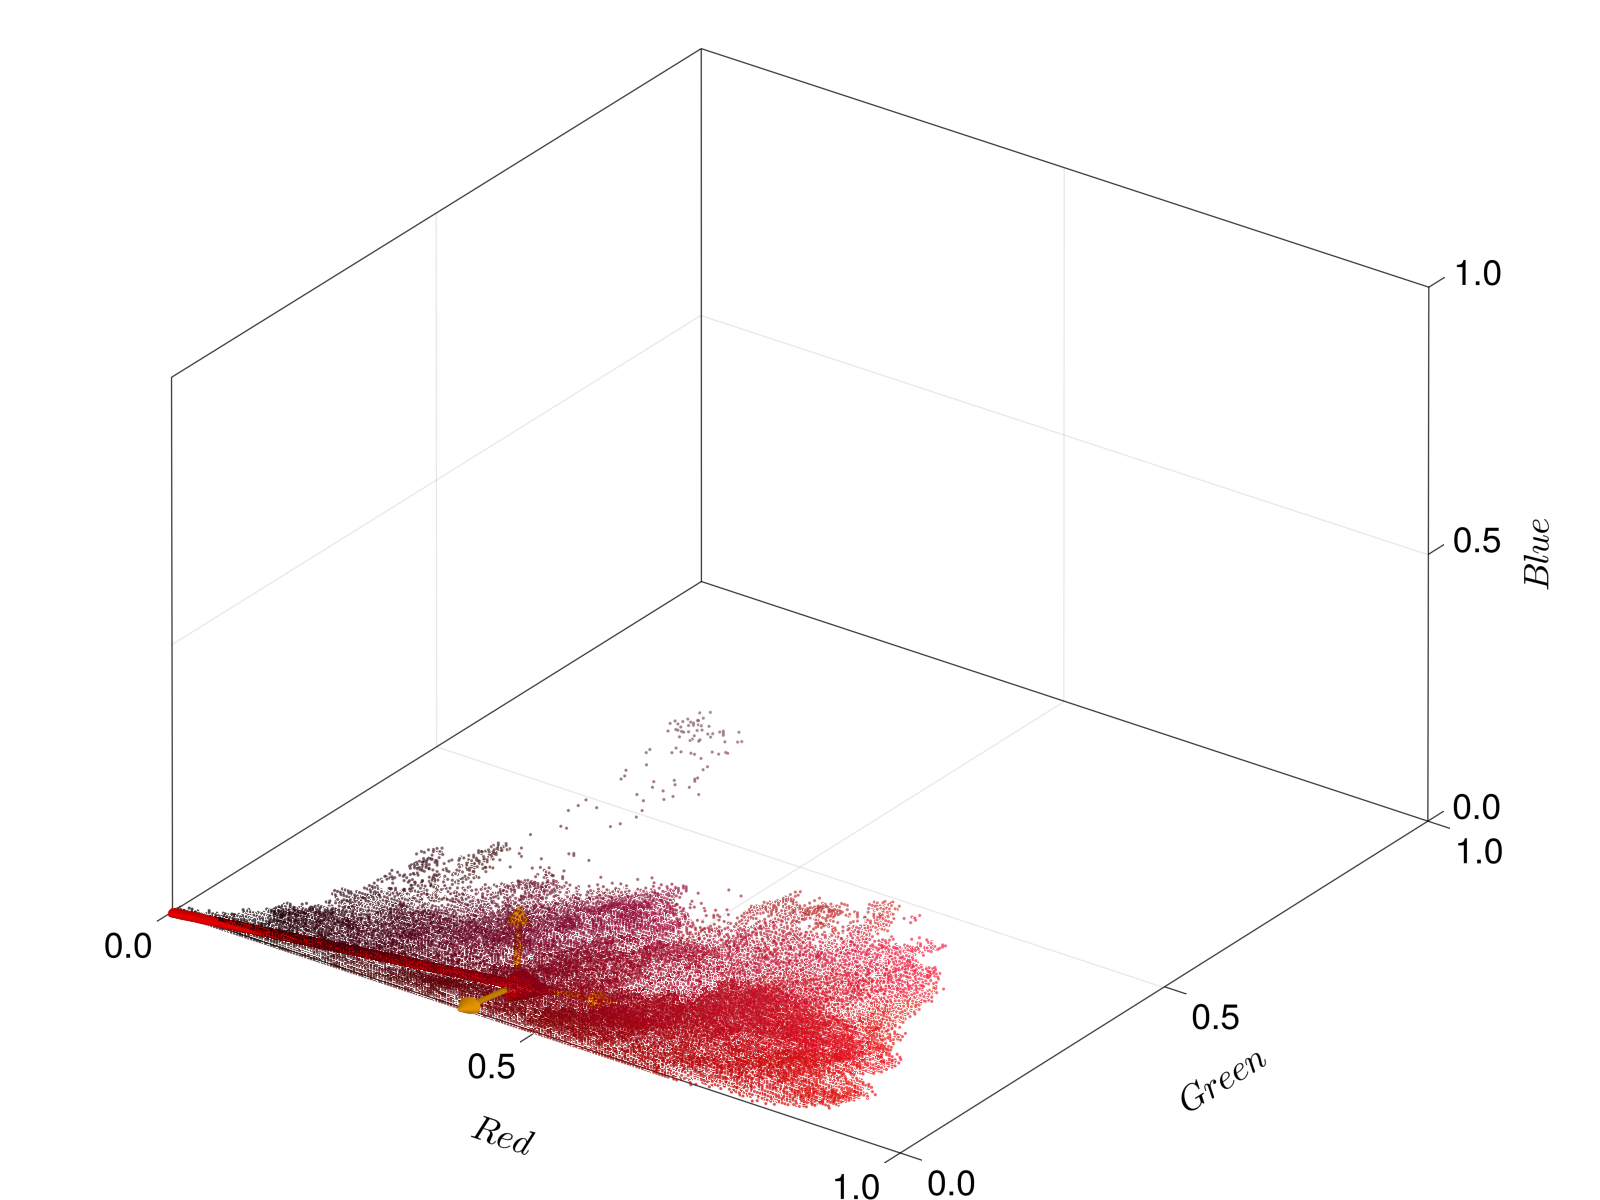
\includegraphics[scale=0.09]{../figures/pixel_cloud_eva_1}
    \end{subfigure}
    \begin{subfigure}[c]{0.3\textwidth}
        \centering
        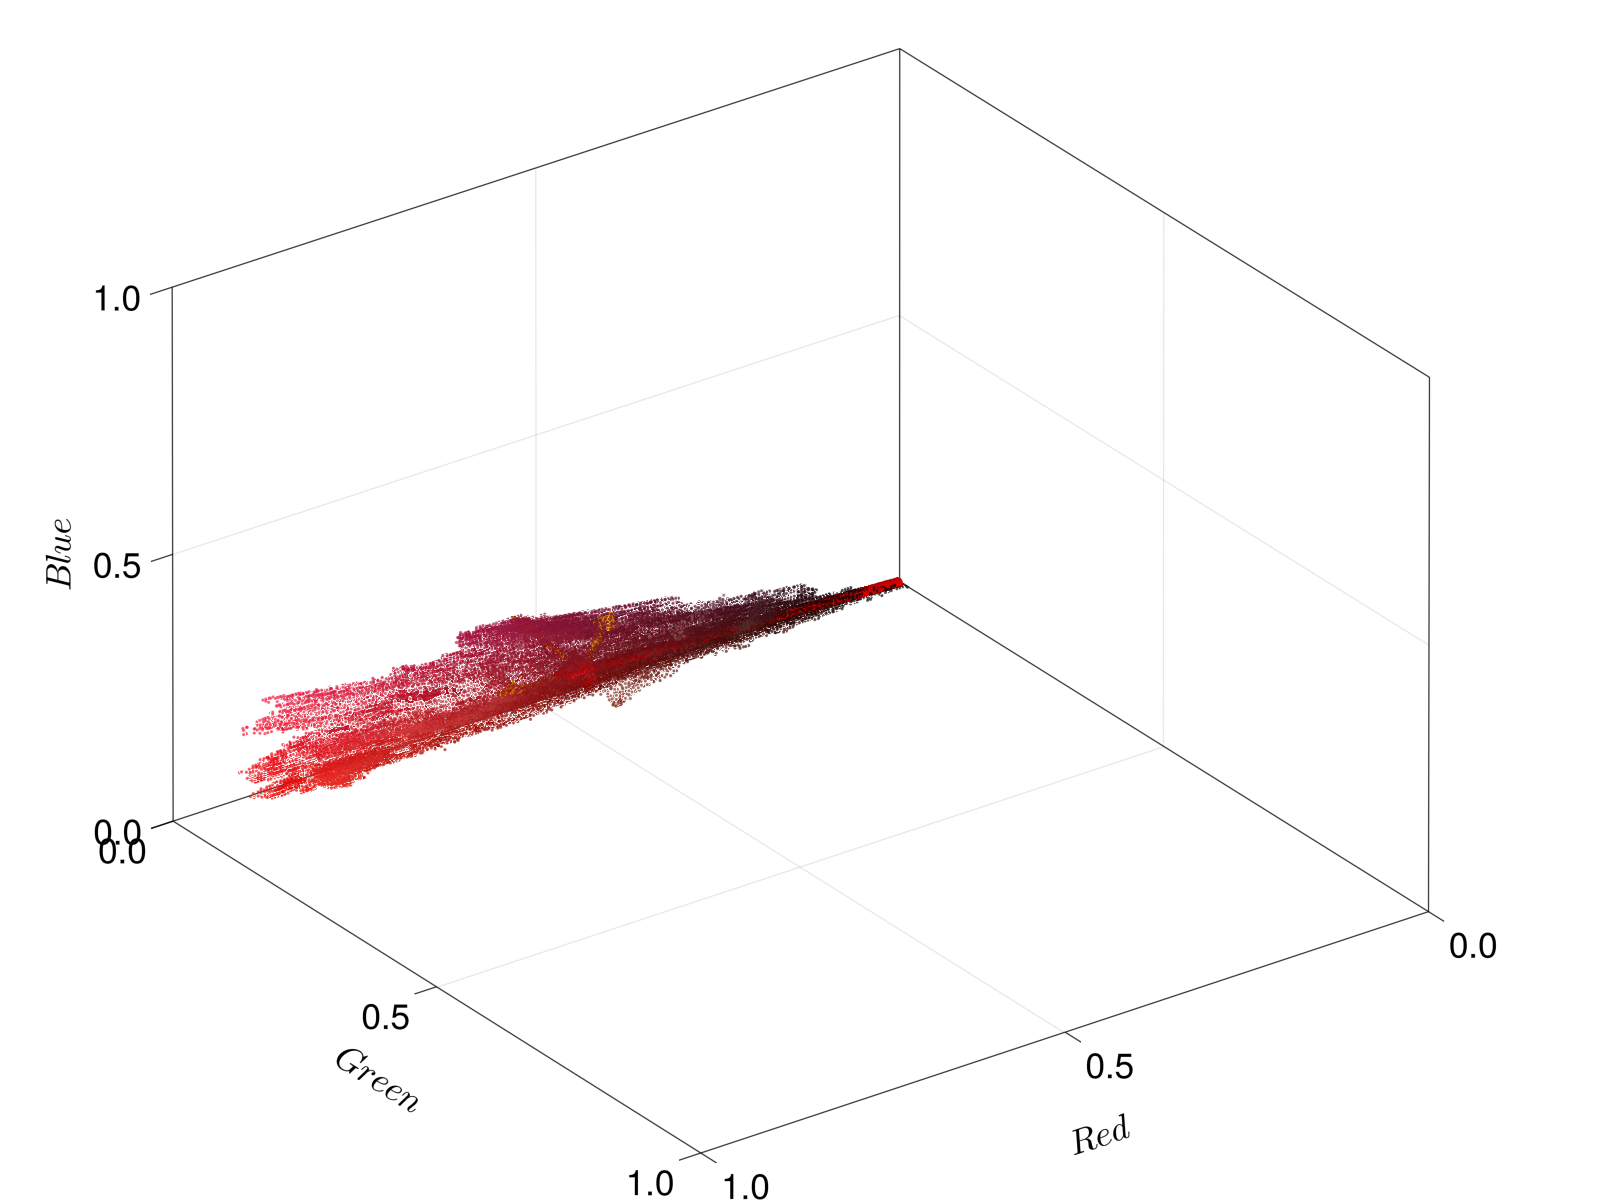
\includegraphics[scale=0.09]{../figures/pixel_cloud_eva_2}
    \end{subfigure}
    \begin{subfigure}[c]{0.3\textwidth}
        \centering
        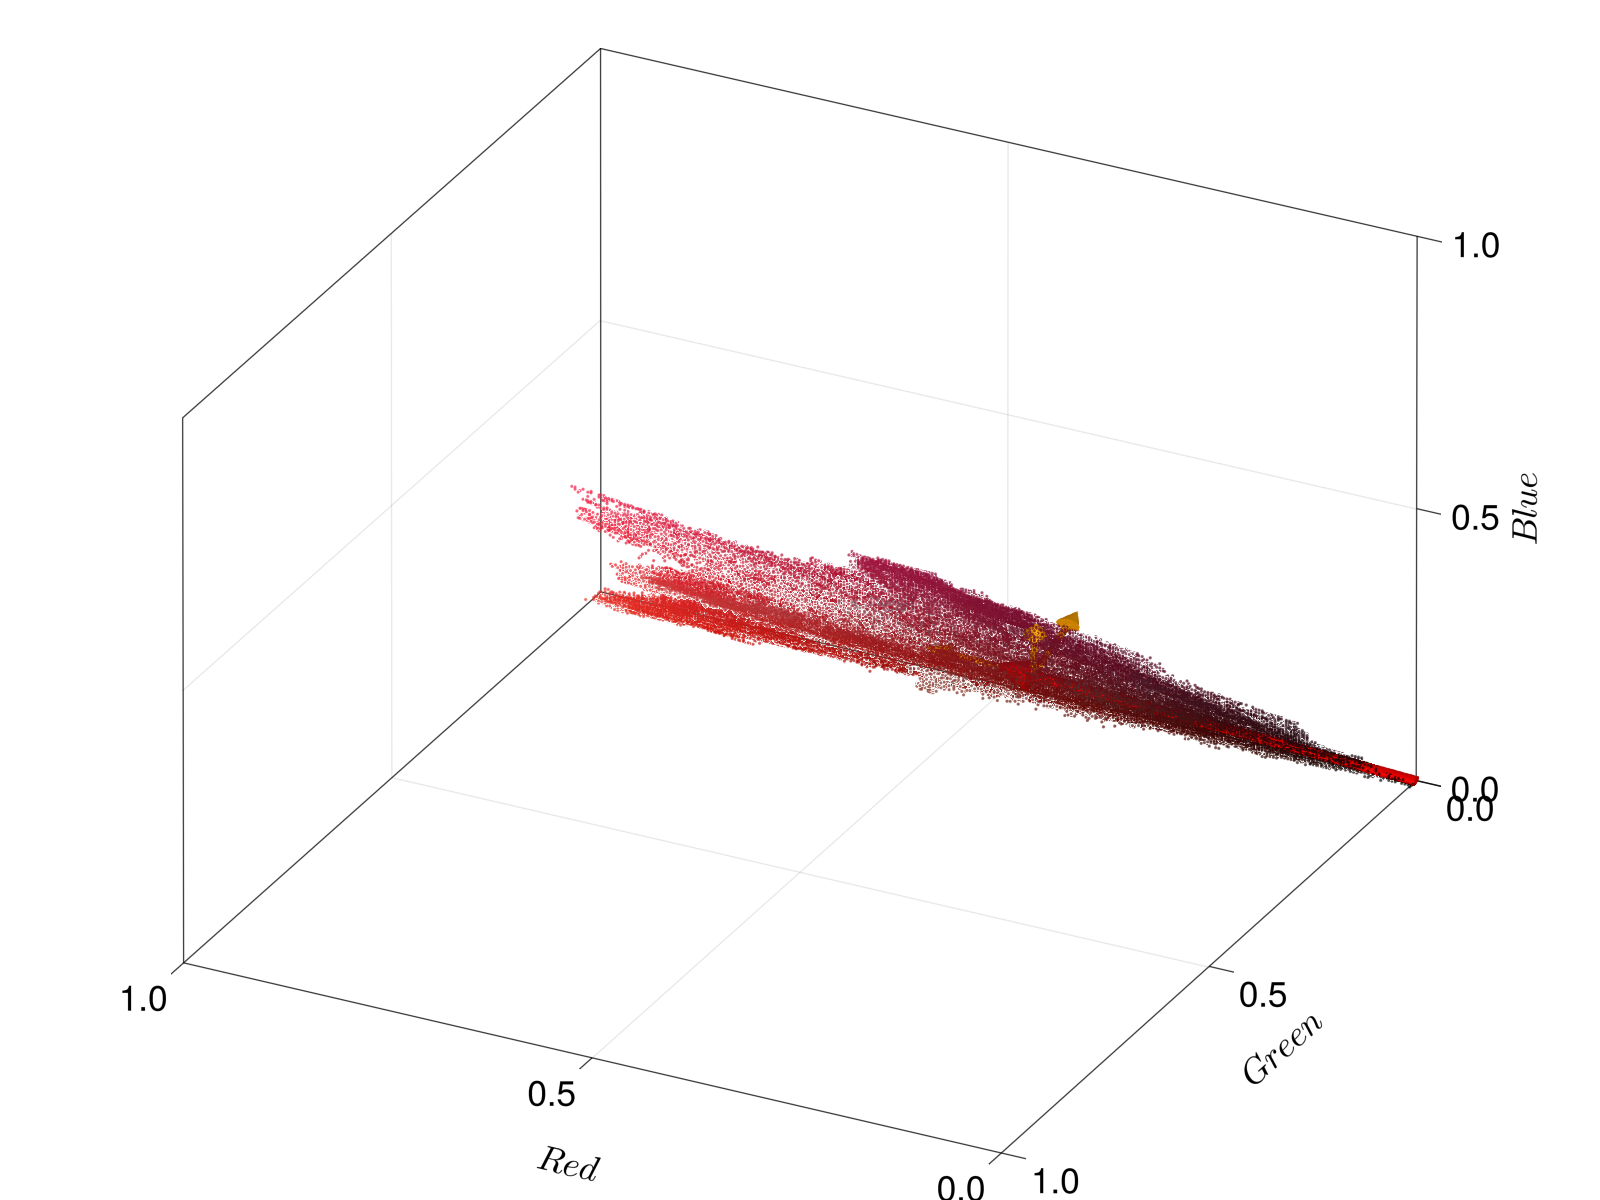
\includegraphics[scale=0.09]{../figures/pixel_cloud_eva_3}
    \end{subfigure}
    \caption{Nubes de pixeles para la \cref{fig:evangelion} con angulos de rotación para las vistas respecto al eje-$Blue$ de $-0.3\pi$, $0.3\pi$ y $0.65\pi$, respectivamente.}
    \label{fig:nube-pixeles-eva}
\end{figure}

De igual manera se incluyó la nube gaussiana de probabilidad para esta imagen, mostrada en la \cref{fig:nube-gaussiana-eva}. Este comportamiento era de esperarse al observar la \cref{fig:nube-pixeles-eva}, la probabilidad se encuentra concentrada alrededor de la zona para pixeles de tonalidades alrededor de los rojos.
\begin{figure}[ht!]
    \centering
    \begin{subfigure}[c]{0.3\textwidth}
        \centering
        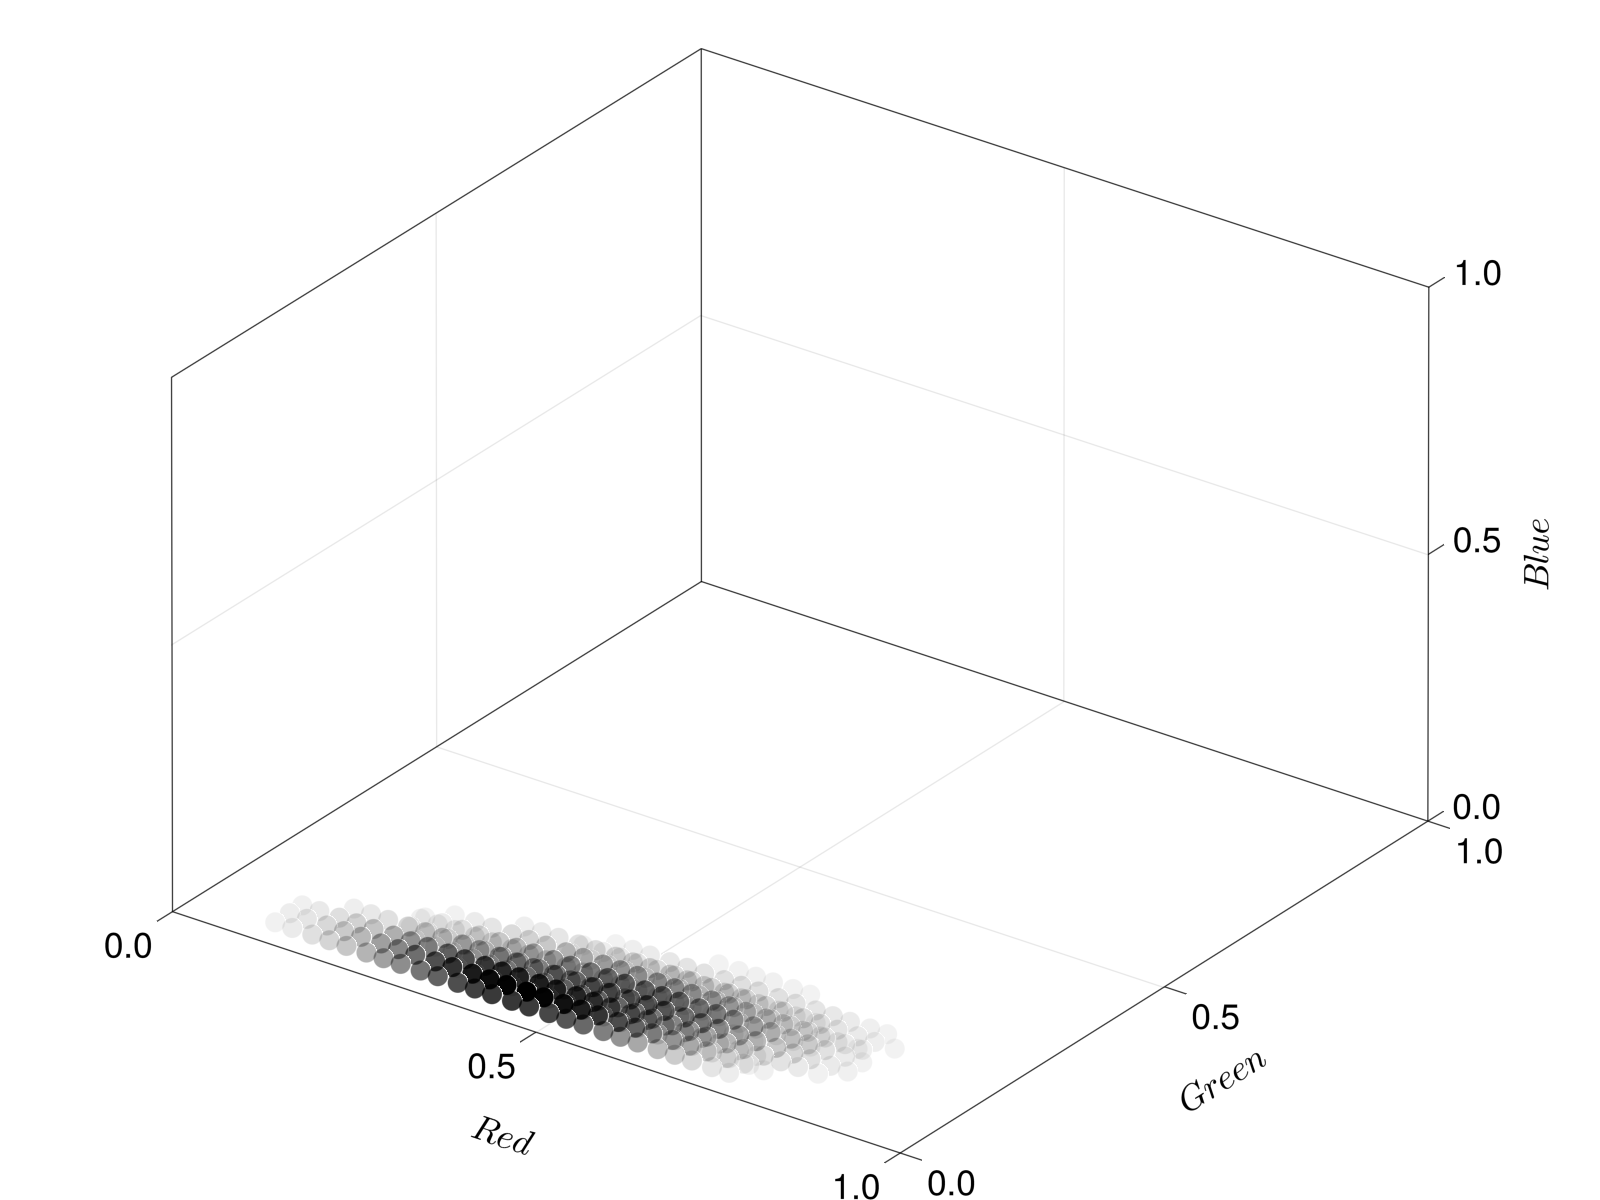
\includegraphics[scale=0.09]{../figures/gaussian_cloud_eva_1}
    \end{subfigure}
    \begin{subfigure}[c]{0.3\textwidth}
        \centering
        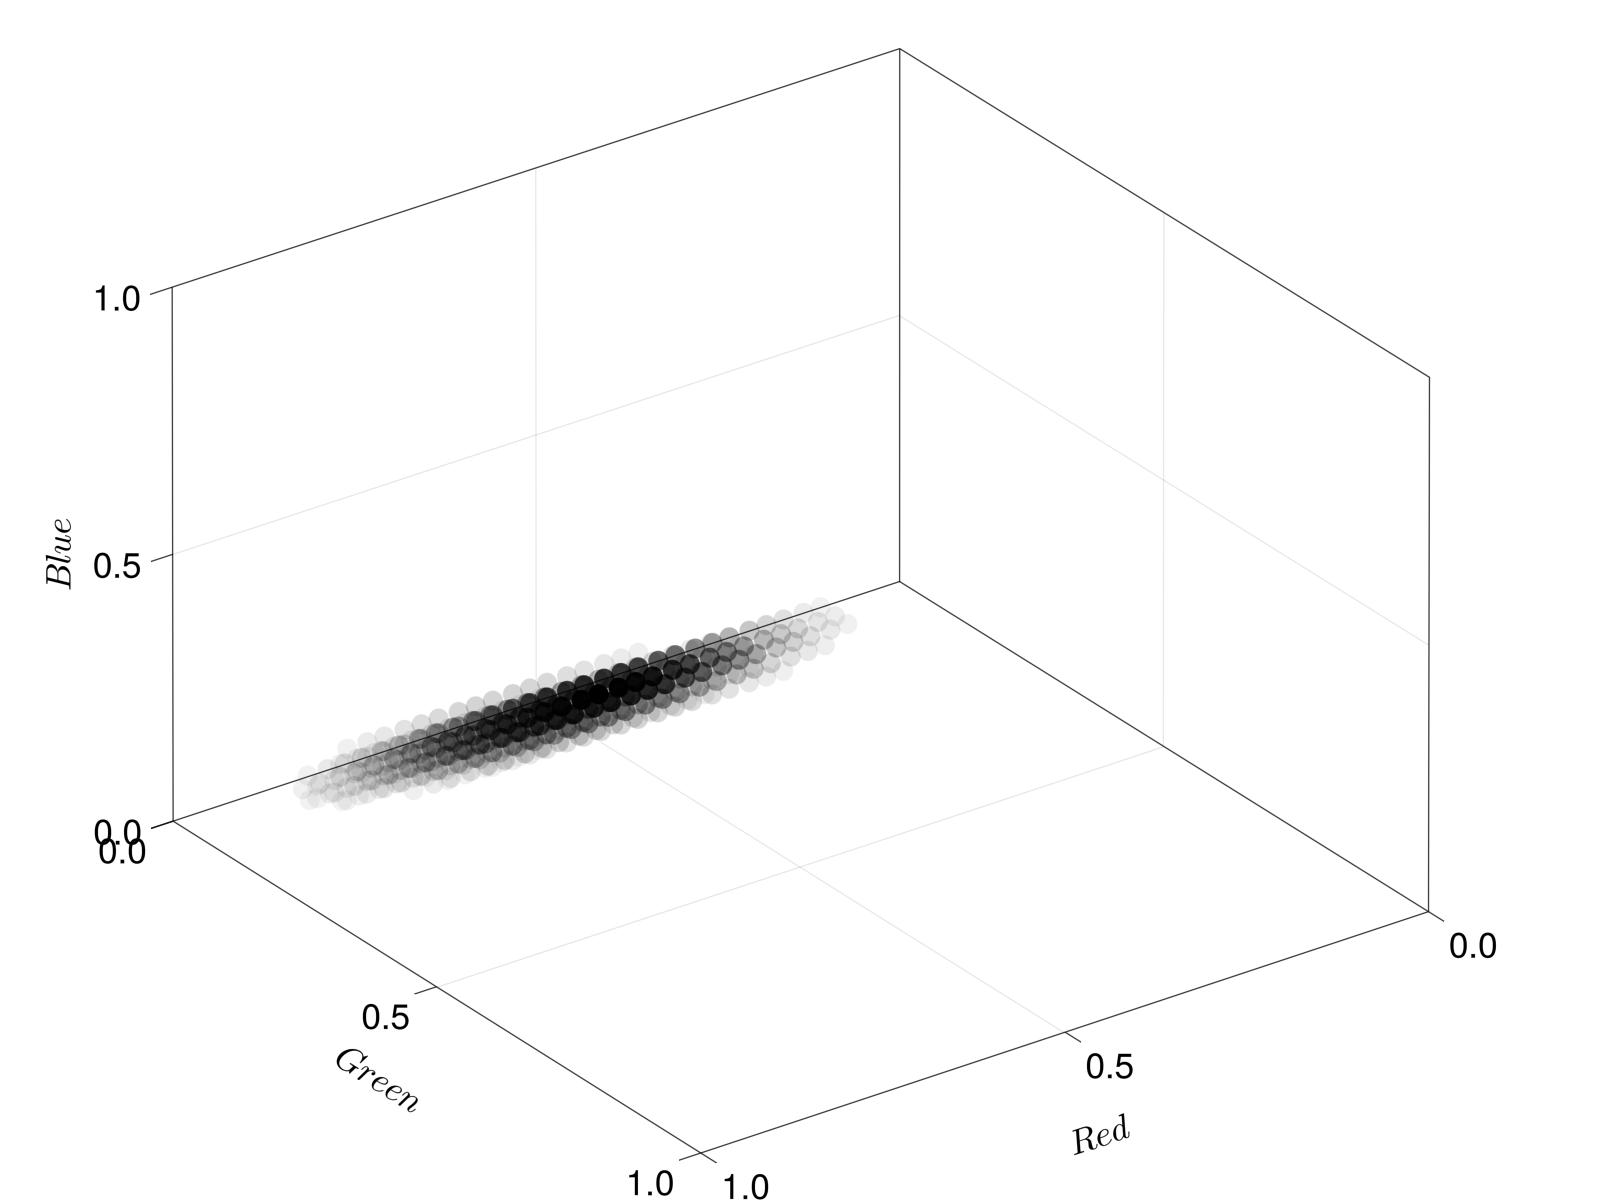
\includegraphics[scale=0.09]{../figures/gaussian_cloud_eva_2}
    \end{subfigure}
    \begin{subfigure}[c]{0.3\textwidth}
        \centering
        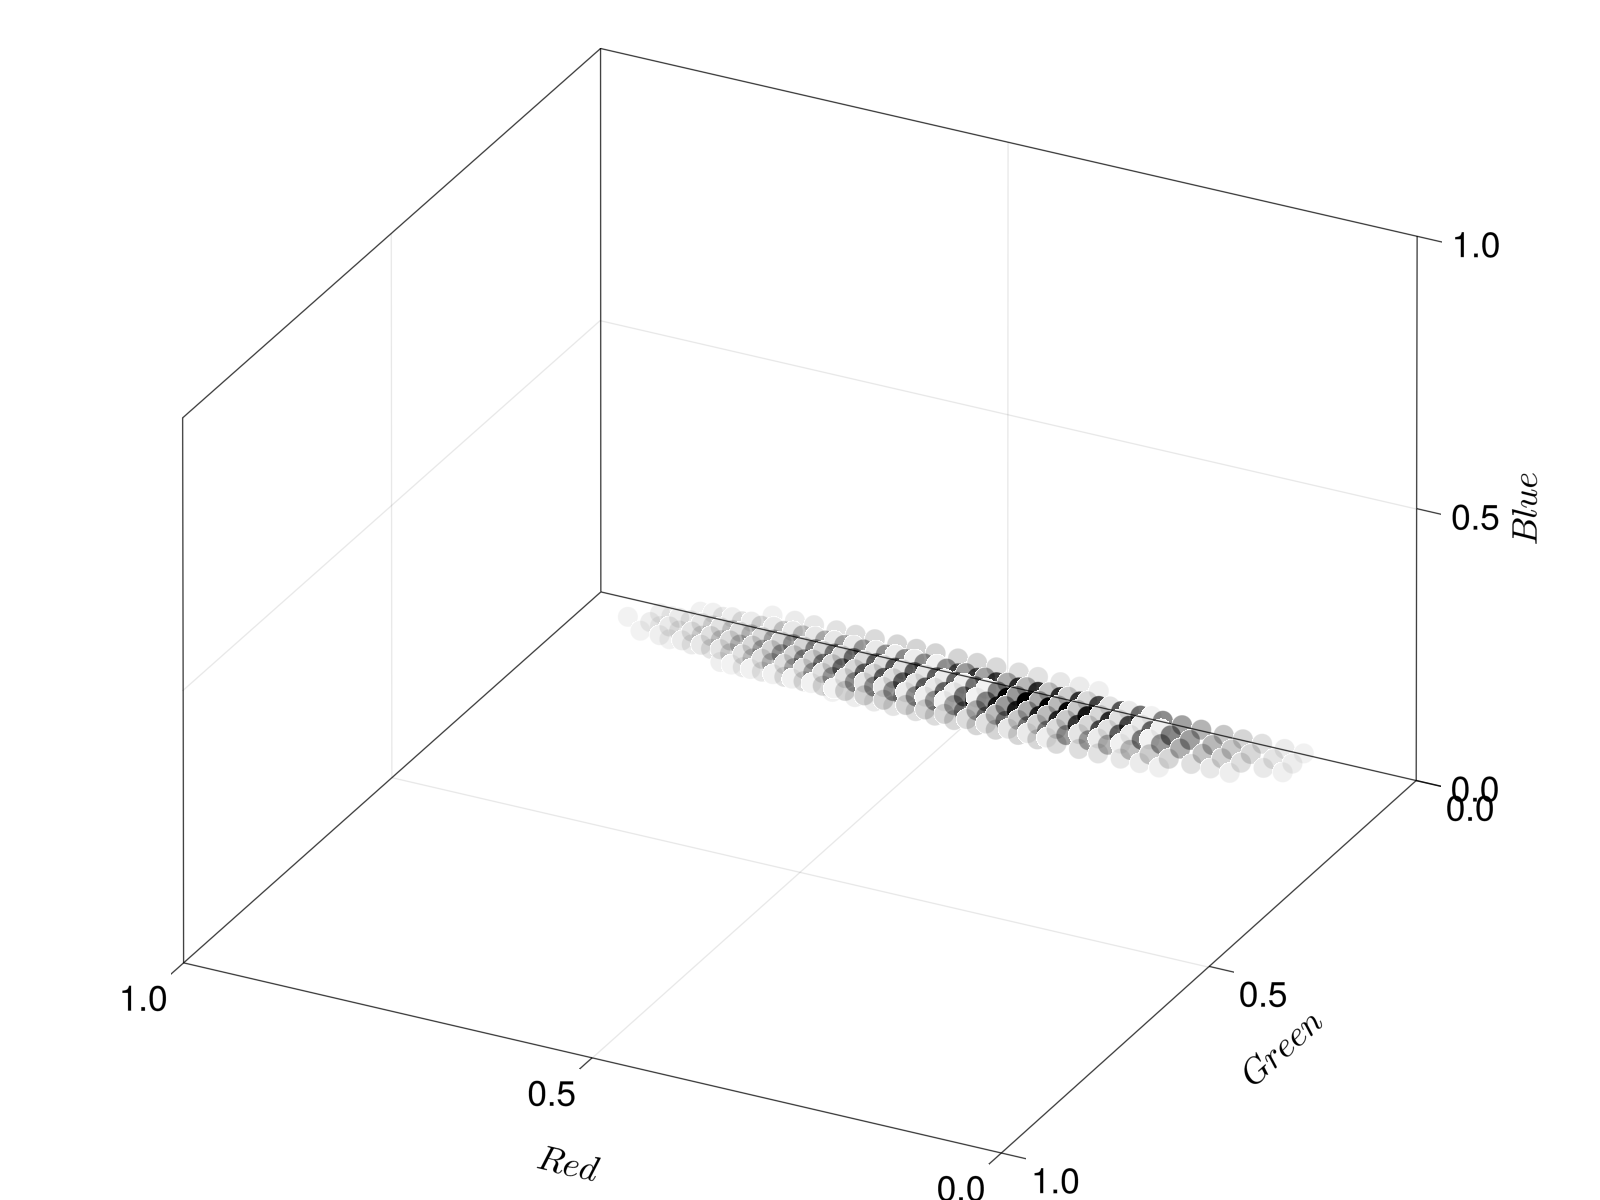
\includegraphics[scale=0.09]{../figures/gaussian_cloud_eva_3}
    \end{subfigure}
    \caption{Nubes de probabilidad para la \cref{fig:evangelion}, donde se muestran con una rotación respecto al eje-$Blue$ de $-0.3\pi$, $0.3\pi$, y $0.65\pi$, respectivamente.}x
    \label{fig:nube-gaussiana-eva}
\end{figure}

Basando en motivos de relevancia social histórica las monorías racializadas \cite{wevers2016kodak} han recibido un trato poco preferente dentro del desarrollo tecnológico. Debido a esto, la última imagen que se decidió usar para completar con los requerimientos de la tarea fue una imagen que incluyera caras de \href{https://guardian.ng/opinion/humanism-and-its-possibilities-in-africa/}{niños originarios de Nigeria}\footnote{No se encontró al fotógrafo de la imagen, los derechos de la imagen no pertenecen a al autor de este trabajo. En el trabajo presente sólamente se usó esta imagen para fines educativos sin fines de lucro}.
\begin{figure}[ht!]
    \centering
    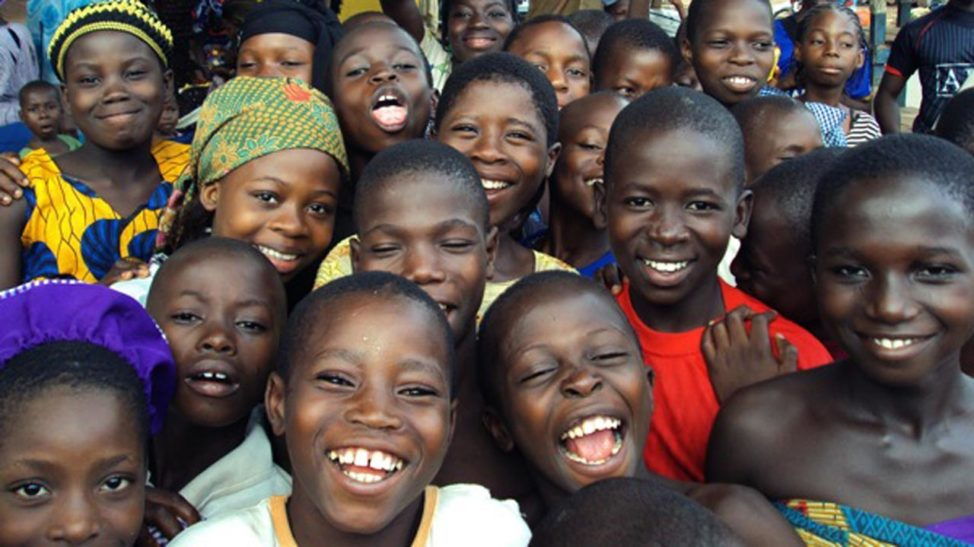
\includegraphics[scale=0.25]{../figures/nigerian-children}
    \caption{Caras de niños originarios de Nigeria.}
    \label{fig:kids}
\end{figure}

Las dimensiones de la imagen mostrada en la \cref{fig:kids} son de $(547, 974)$, y cuenta con aproximadamente $5.3E5$ pixeles. El vector promedio $\vec{m}_4$, la matriz de correlación $\Sigma_4$ y la matriz de covarianza $R_4$ son
\begin{align*}
    \vec{m}_4 & =
    \begin{bmatrix}
        0.3739 \\
        0.3188 \\
        0.3042
    \end{bmatrix}, &
    \Sigma_4 & =
    \begin{bmatrix}
        0.0565 & 0.0452 & 0.0304 \\
        0.0452 & 0.0476 & 0.0351 \\
        0.0304 & 0.0351 & 0.0392
    \end{bmatrix}, &
    R_4 & = 
    \begin{bmatrix}
        1.0    & 0.8716 & 0.6474 \\
        0.8716 & 1.0    & 0.8128 \\
        0.6474 & 0.8128 & 1.0
    \end{bmatrix}.
\end{align*}

Los eigenvalores de $\Sigma_4$ son $\lambda_1 = 0.0002$, $\lambda_2 = 0.0022$, $\lambda_3 = 0.0351$, y sus respectivos eigenvectores son
\begin{align*}
    \vec{s_1} & =
    \begin{bmatrix}
        0.4516 \\
        -0.7954 \\
         0.4040
    \end{bmatrix}, &
    \vec{s_2} & = 
    \begin{bmatrix}
        0.6292 \\
        -0.0371 \\
        -0.7763
    \end{bmatrix}, &
    \vec{s_3} & =
    \begin{bmatrix}
        0.6325 \\
        0.6049 \\
        0.4837 \\
    \end{bmatrix}.
\end{align*}

Finalmente, en la \cref{fig:nube-pixeles-kids,fig:nube-gaussiana-kids} se muestran las nubes de pixeles y de probabilidad, respectivamente.
\begin{figure}[ht!]
    \centering
    \begin{subfigure}[c]{0.3\textwidth}
        \centering
        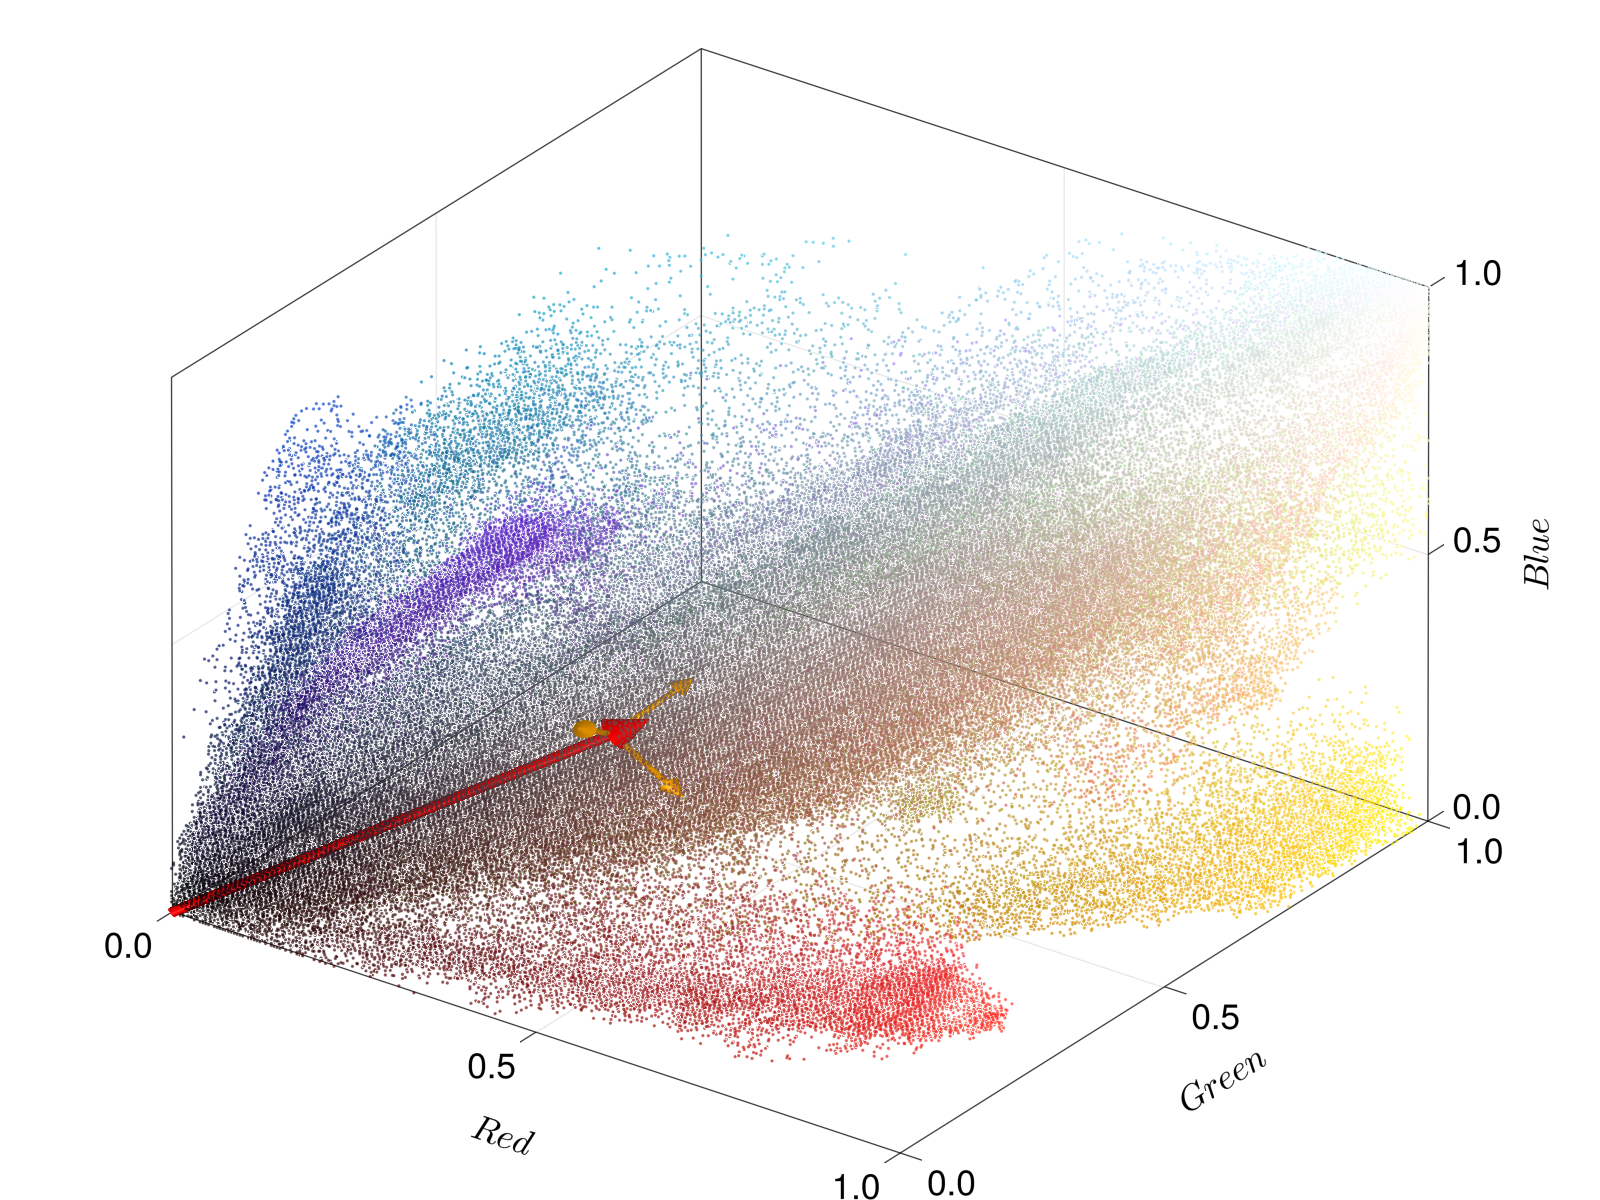
\includegraphics[scale=0.09]{../figures/pixel_cloud_kids_1}
    \end{subfigure}
    \begin{subfigure}[c]{0.3\textwidth}
        \centering
        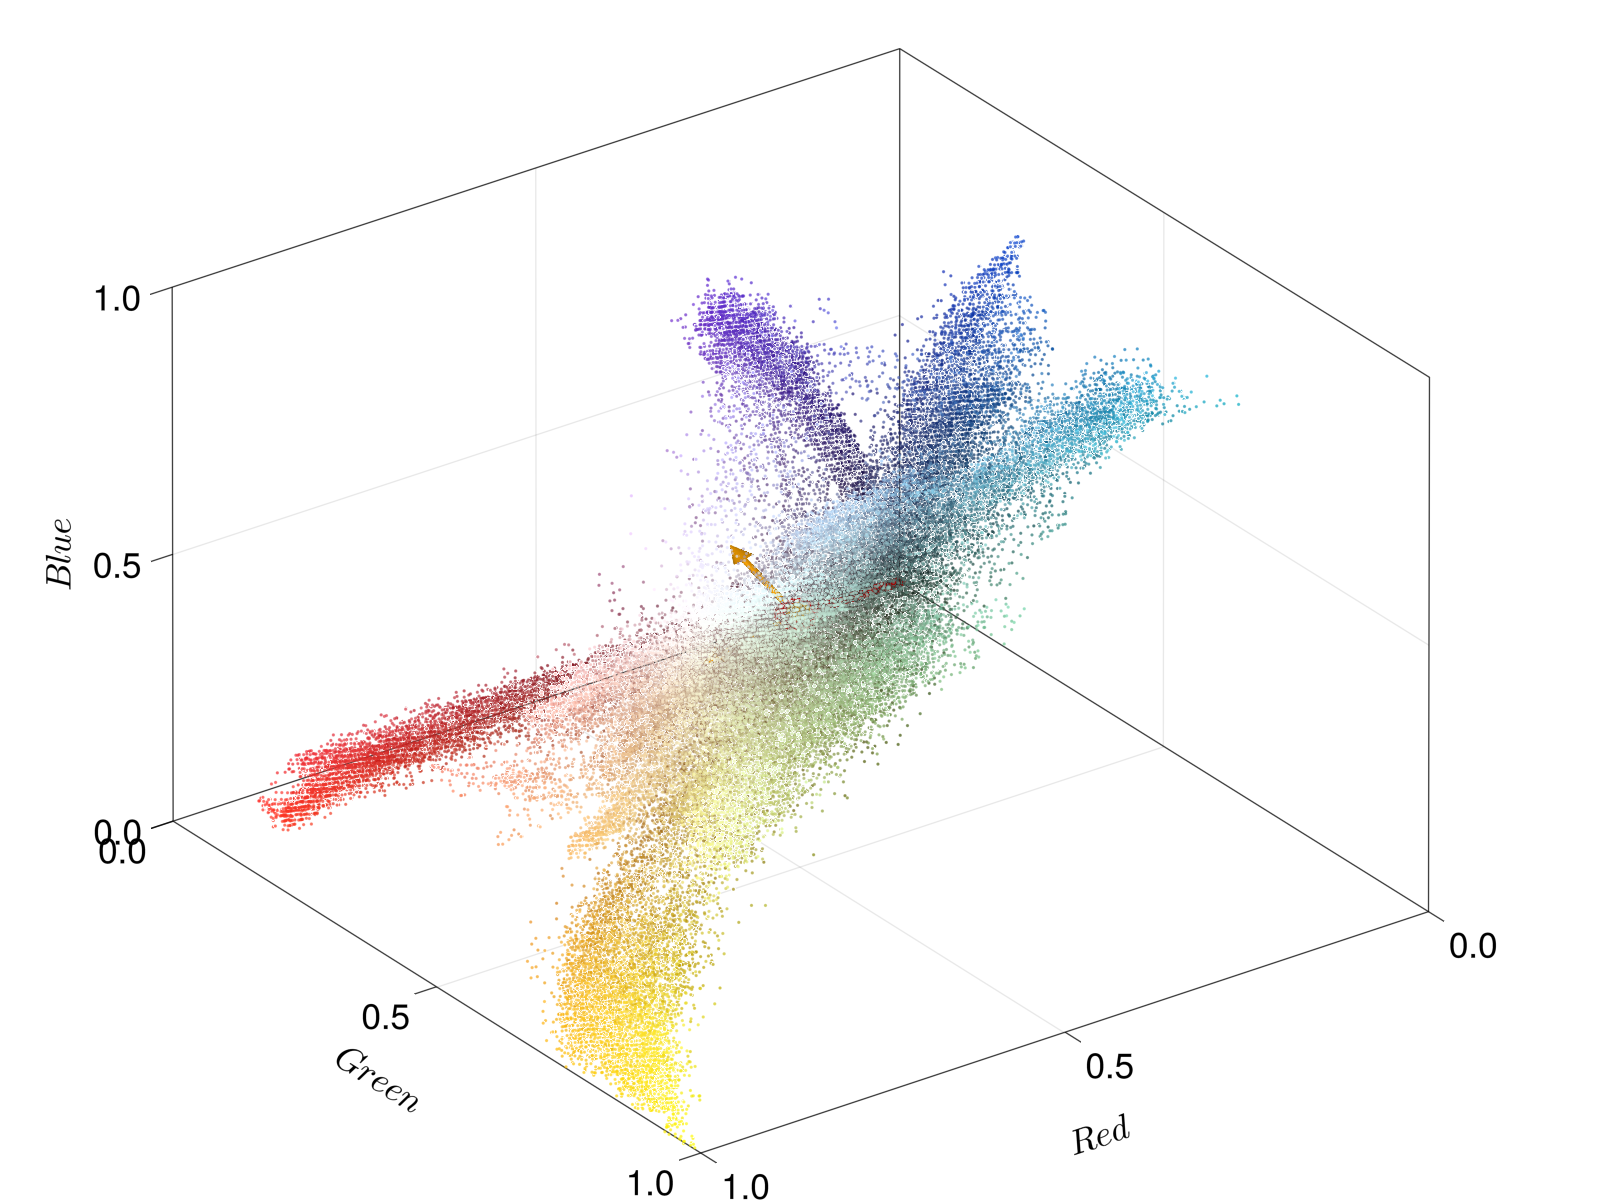
\includegraphics[scale=0.09]{../figures/pixel_cloud_kids_2}
    \end{subfigure}
    \begin{subfigure}[c]{0.3\textwidth}
        \centering
        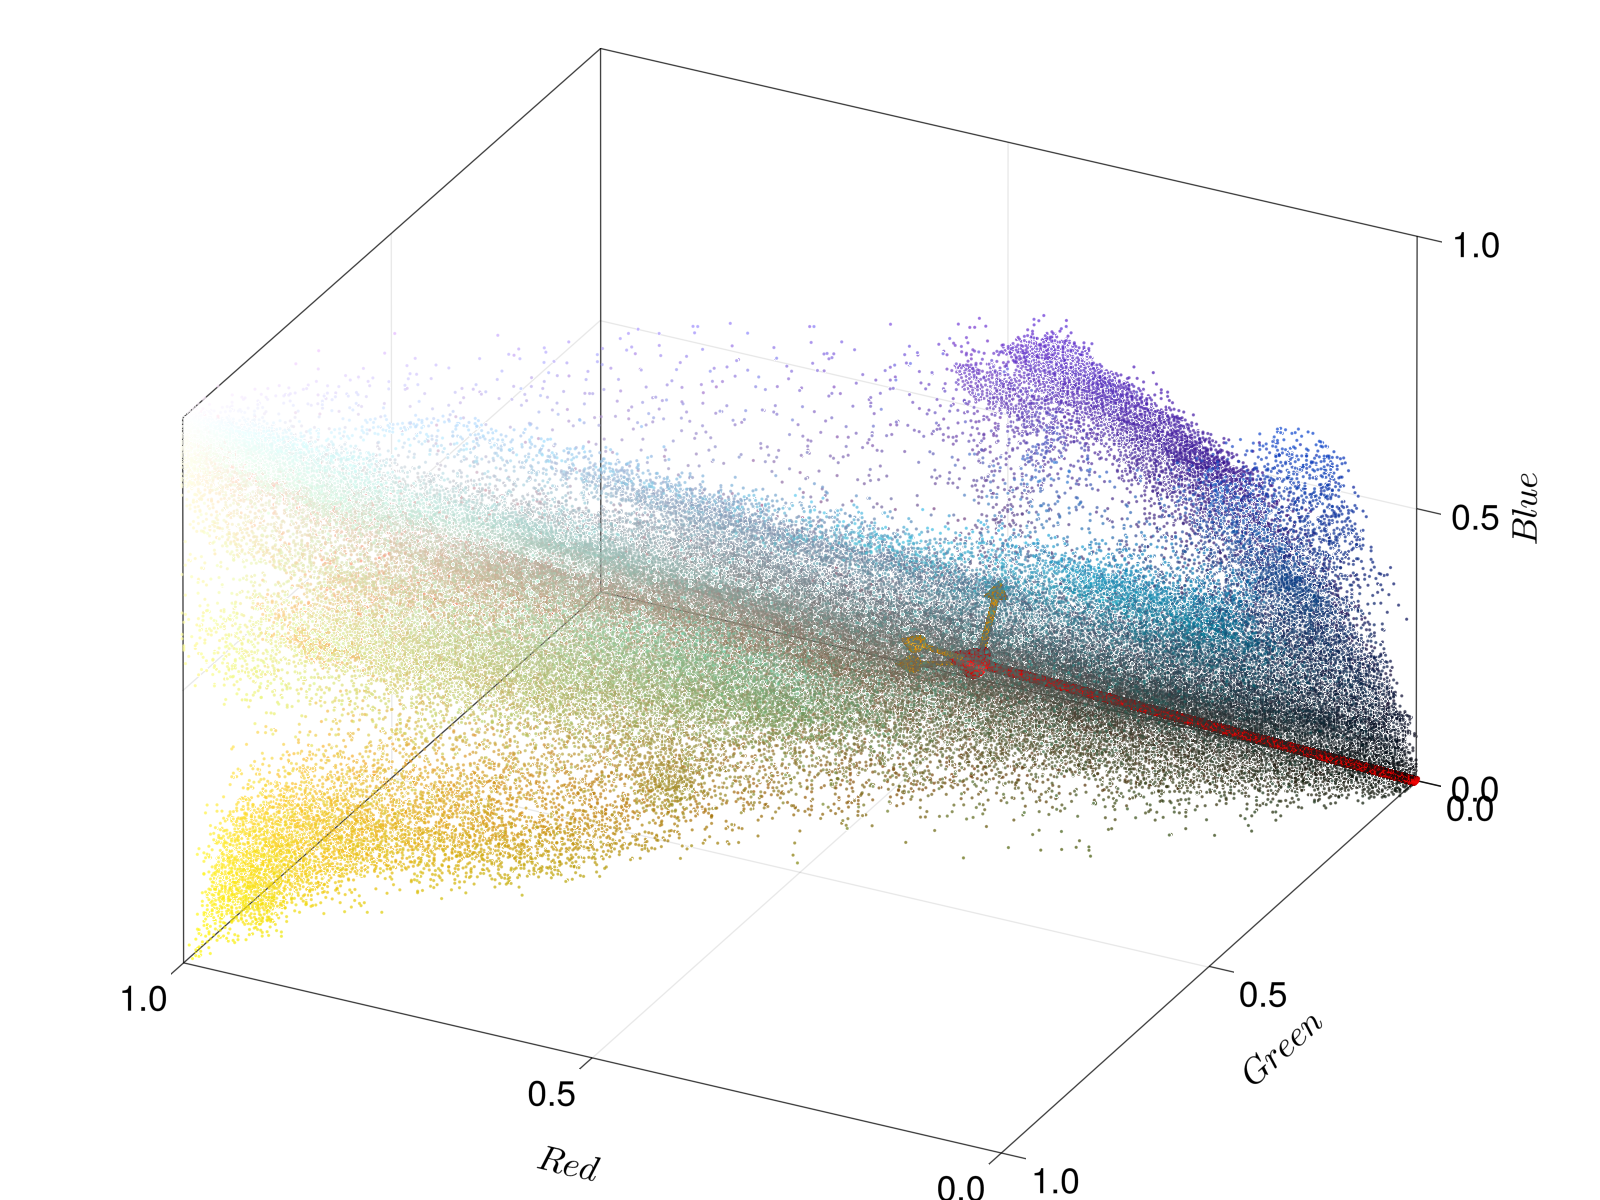
\includegraphics[scale=0.09]{../figures/pixel_cloud_kids_3}
    \end{subfigure}
    \caption{Nubes de pixeles para la \cref{fig:kids} con angulos de rotación para las vistas respecto al eje-$Blue$ de $-0.3\pi$, $0.3\pi$ y $0.65\pi$, respectivamente.}
    \label{fig:nube-pixeles-kids}
\end{figure}

\begin{figure}[ht!]
    \centering
    \begin{subfigure}[c]{0.3\textwidth}
        \centering
        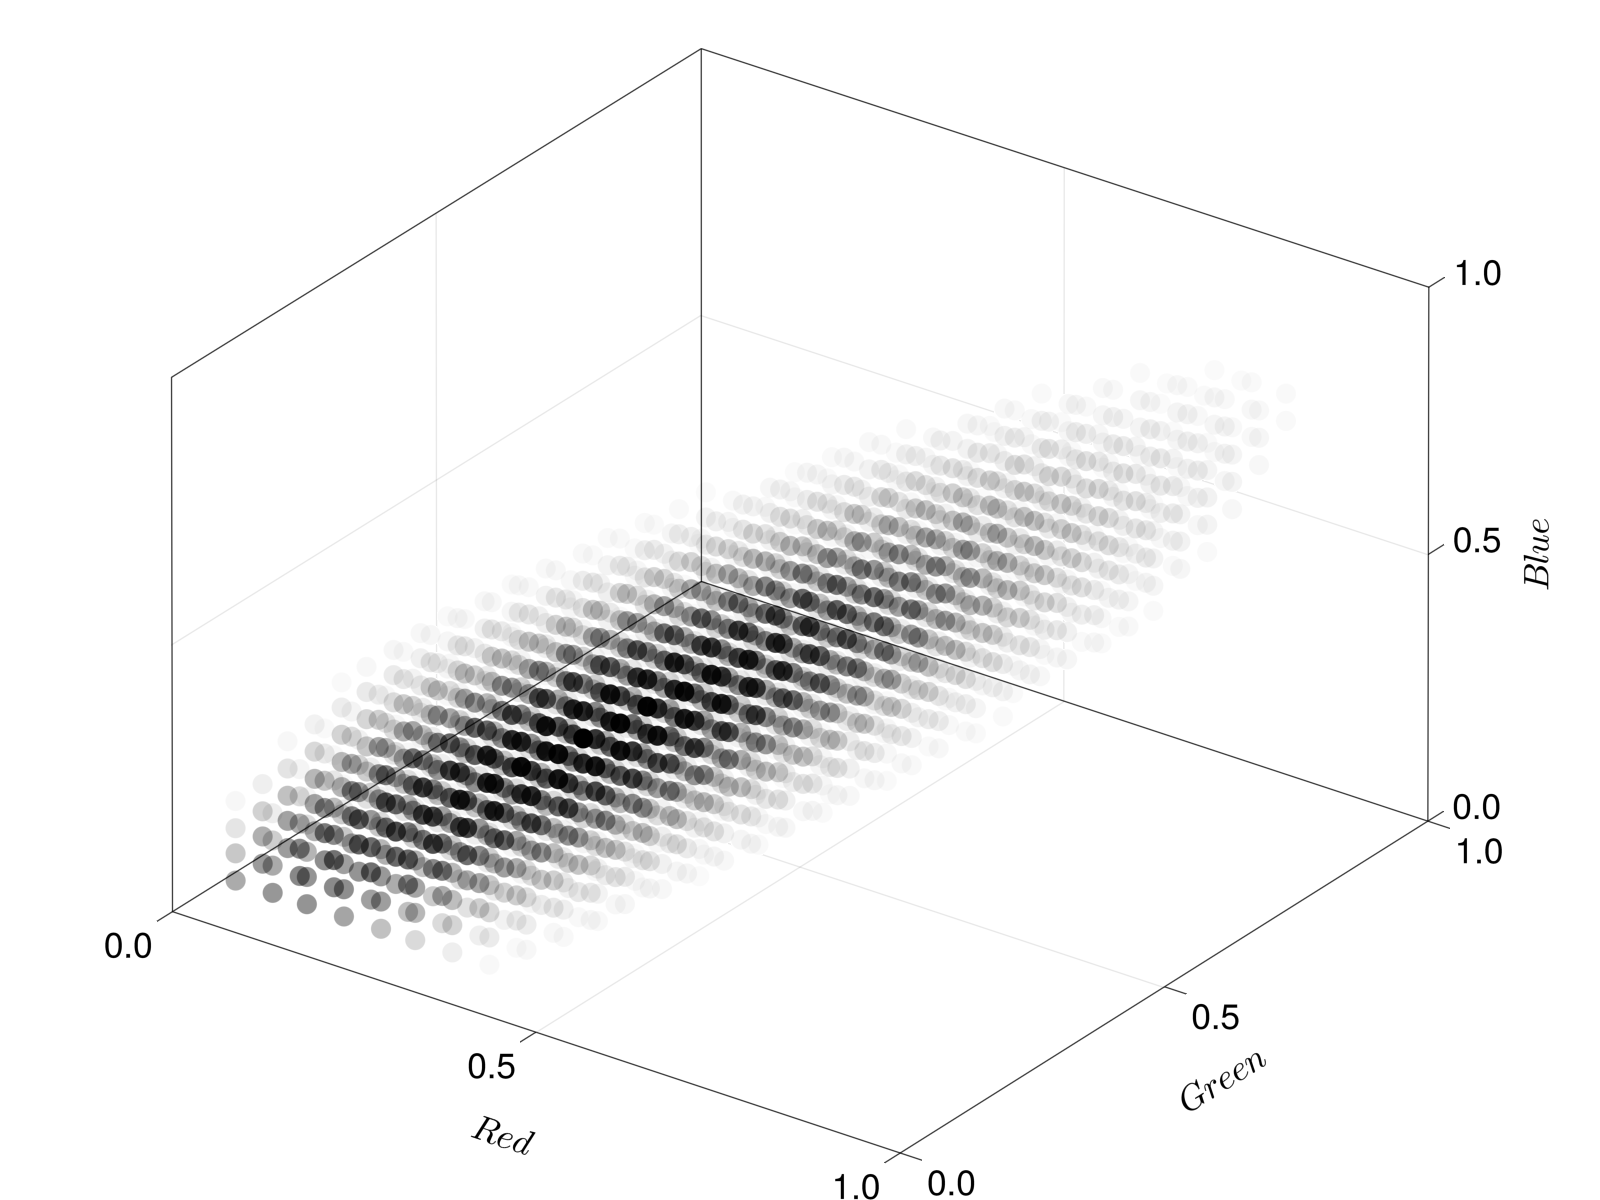
\includegraphics[scale=0.09]{../figures/gaussian_cloud_kids_1}
    \end{subfigure}
    \begin{subfigure}[c]{0.3\textwidth}
        \centering
        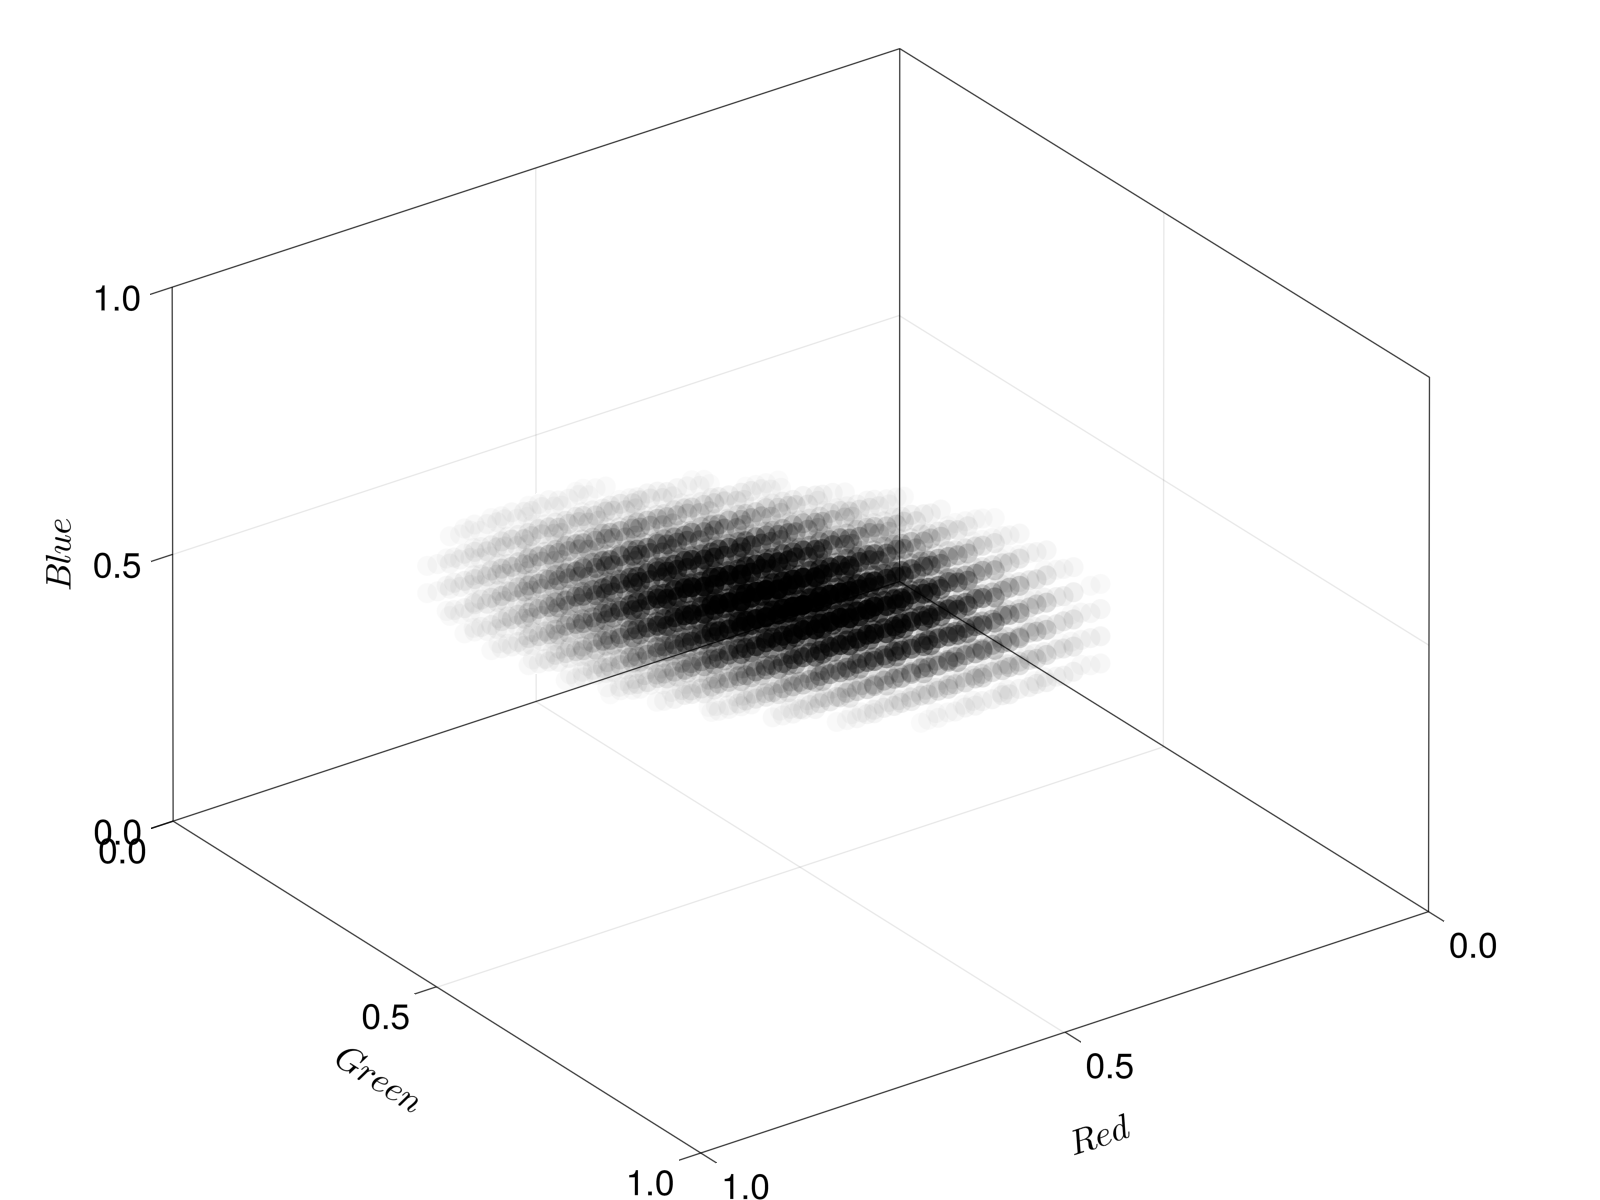
\includegraphics[scale=0.09]{../figures/gaussian_cloud_kids_2}
    \end{subfigure}
    \begin{subfigure}[c]{0.3\textwidth}
        \centering
        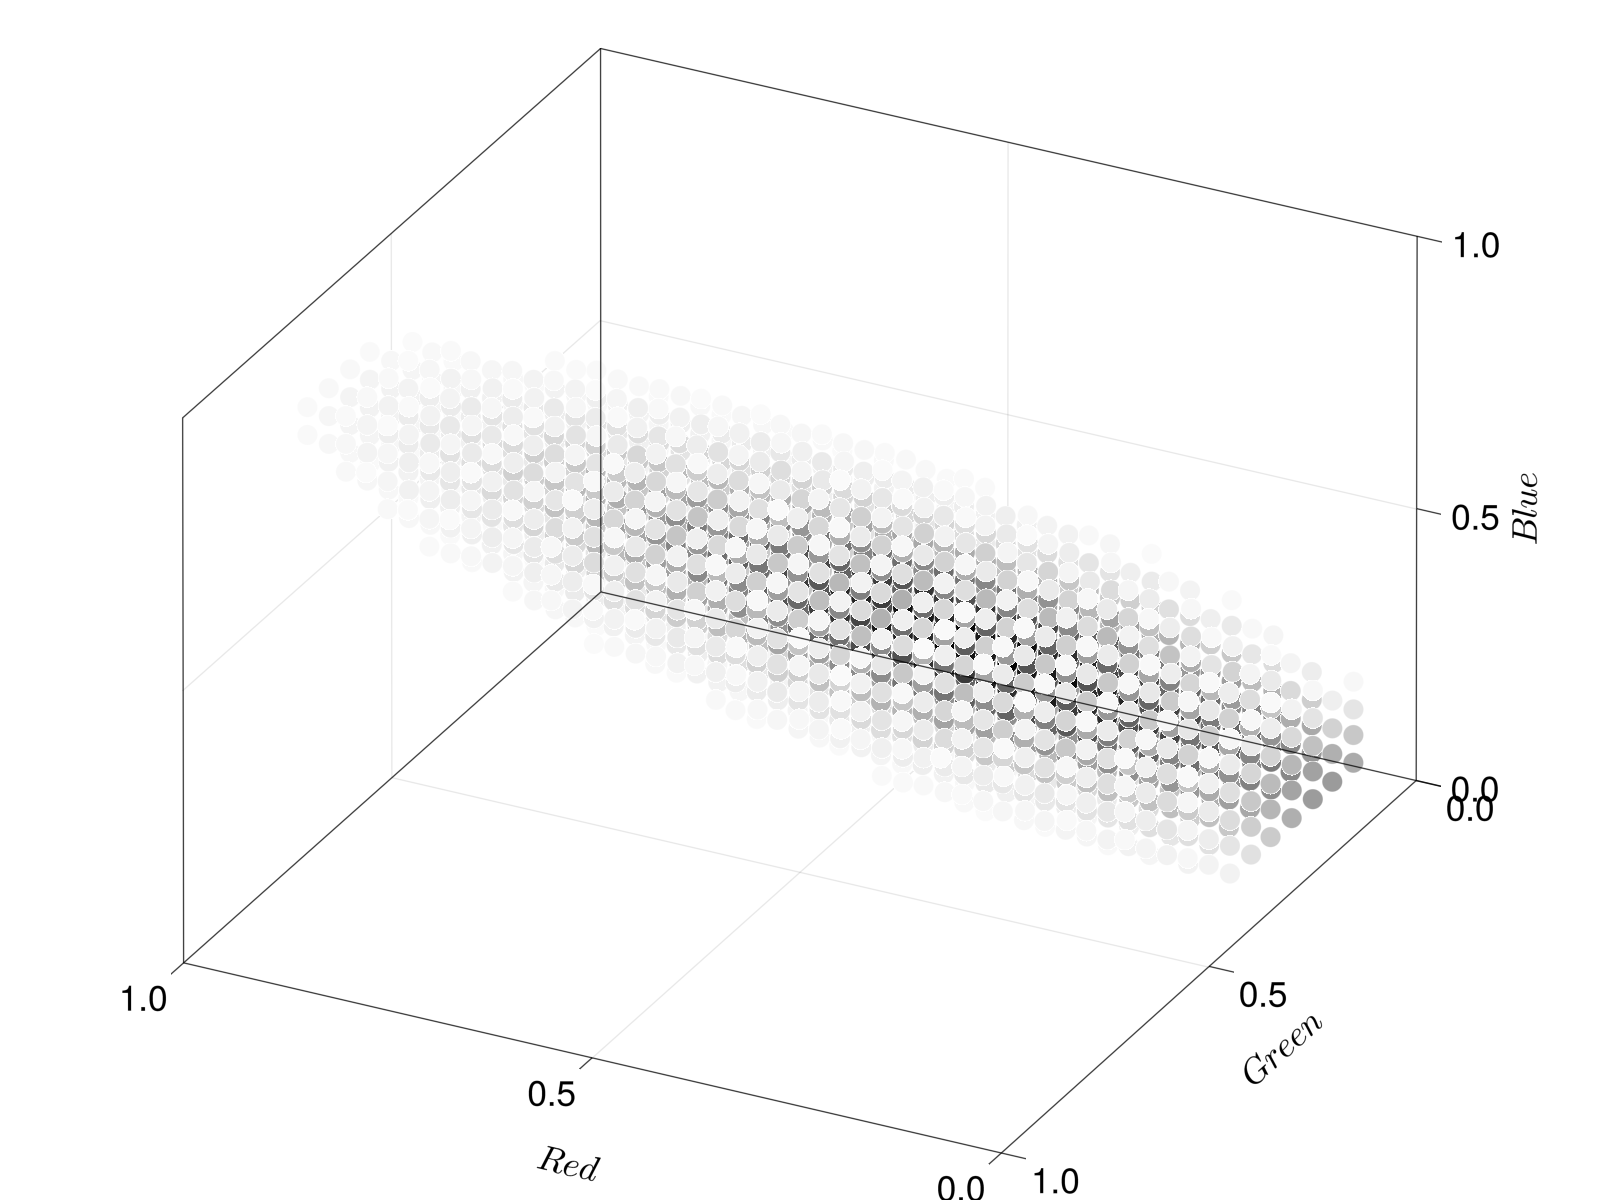
\includegraphics[scale=0.09]{../figures/gaussian_cloud_kids_3}
    \end{subfigure}
    \caption{Nubes de probabilidad para la \cref{fig:kids}, donde se muestran con una rotación respecto al eje-$Blue$ con ángulos de $-0.3\pi$, $0.3\pi$, y $0.65\pi$, respectivamente.}
    \label{fig:nube-gaussiana-kids}
\end{figure}

Tiene sentido pensar que las nubes de probabilidad gaussianas se localizen en alrededor de la posición del vector promedio y además que se extiendan a ocupar las posiciones de sus nubes de pixeles. No se puede apreciar si dichas nubes gaussianas presentan rotaciones sobre los ejes de sus vectores promedio $\vec{m}_i$ pero se espera que este sea el caso debido a que deberian de expandirse en las direcciones de sus respectivos eigenvectores. Nótese que los eigenvectores, en todos los casos, fueron escalados por un factor de $1/10$ en las visualizaciones únicamente.

Se desarrolló un pequeño módulo para analizar imágenes usando el lengauge de programación \textit{Julia} \cite{Bezanson_Julia_A_fresh_2017} basándose en la teoría vista en clase, y en el libro añadido en las referencias \cite{richards2006remote}. Adicionalmente, las visualizaciones se realizaron usando la librería \textit{GLMakie} \cite{DanischKrumbiegel2021}, también parte de \textit{Julia}.

\pagebreak

\nocite{*} % to call all references even if they are not cited in the text
\bibliography{references.bib}

\pagebreak

\vspace{1cm}
\section*{Apéndice}
\inputminted[
    frame=none,
    % obeytabs=false,
    breaklines,
    tabsize=4,
    linenos=true,
    % numbersep=-10pt,
    baselinestretch=1,
    firstnumber=last,
    bgcolor=bg,
]{julia}{\codepath}


\end{document}